\chapter{Extrapolating Volition with Recursive Information Markets}
\label{chap:recursive-information-markets}

\chapterprovenance{Adapted from ``Extrapolating Volition with Recursive
Information Markets'' by Abhimanyu Pallavi Sudhir and Long Tran-Thanh.}

\providecommand{\Nats}{\mathbb{N}}
\providecommand{\Ints}{\mathbb{Z}}
\NewDocumentCommand{\sigalg}{}{\mathcal{F}}
\NewDocumentCommand{\sigalgalt}{}{\mathcal{G}}
\NewDocumentCommand{\Probof}{m}{\Prob\left[#1\right]}
\NewDocumentCommand{\Expect}{}{\mathbf{E}}
\NewDocumentCommand{\Expectof}{m}{\Expect\left[#1\right]}
\NewDocumentCommand{\Expectofu}{o m}{\Expect_{#1}\left[#2\right]}
\NewDocumentCommand{\Powerset}{m}{\mathcal{P}\left(#1\right)}
\NewDocumentCommand{\Actions}{}{\mathcal{X}}
\NewDocumentCommand{\Samples}{}{\Omega}
\NewDocumentCommand{\Sigalg}{}{\mathcal{F}}
\NewDocumentCommand{\infogood}{}{\mathbf{I}}
\NewDocumentCommand{\zero}{}{\mathbf{0}}
\NewDocumentCommand{\BuyerContext}{}{\textsc{BuyerContext}}
\NewDocumentCommand{\InfoOffer}{}{\textsc{InfoOffer}}
\NewDocumentCommand{\InfoOffers}{}{\textsc{InfoOffers}}
\NewDocumentCommand{\BuyerContexts}{}{\textsc{BuyerContexts}}
\NewDocumentCommand{\Seller}{}{\textsc{Seller}}
\NewDocumentCommand{\Sellers}{}{\textsc{Sellers}}
\NewDocumentCommand{\RIP}{}{\textsc{RIP}}
\NewDocumentCommand{\LLM}{}{\texttt{LLM}}
\NewDocumentCommand{\prompt}{}{\texttt{prompt}}
\NewDocumentCommand{\infooffers}{}{\mathcal{I}}
\NewDocumentCommand{\infonomyurl}{}{\url{https://anonymous.4open.science/r/infonomy-server-5668/}}
\NewDocumentCommand{\infonomy}{}{\texttt{infonomy-server}}
\providecommand{\Struct}[1]{\State \textbf{class} \textsc{#1}}
\providecommand{\EndStruct}{\State \textbf{end class}}
\providecommand{\bleg}[1]{}

\section*{Abstract}
% In typical economic models, the presence of information asymmetry impedes market efficiency, because it means the seller is not incentivized to optimize on features unknown to the buyer. A naive way to approach this may be to

\noindent\textbf{Background:} A key challenge in information economics and AI alignment is that of efficiently valuing or scoring information supplied by a seller or language model that is potentially more-informed than the buyer or evaluator. This is known as the problem of ``information asymmetry'' in economics or ``scalable oversight'' in AI alignment.

% Information markets and human-feedback pipelines face information asymmetry: evaluators can only score what they currently know, which can reward persuasive but incomplete information and misalign incentives.

\noindent\textbf{Objectives and Research Questions:} We ask how to formalize value-of-information under recursive inspection, whether deeper inspection can be made decision-theoretically principled, and how such mechanisms can support scalable oversight beyond standard RLHF.

 \noindent\textbf{Methods:} We introduce a Bayesian framework for recursive information valuation, compare a naive successive protocol to a recursive protocol modeled as an imperfect-recall game, prove ex-ante optimality against admissible protocols, and analyze a marginal-value reward mechanism for scalable oversight within our Bayesian framework.

\noindent\textbf{Results:} We show ex-post inspection alone can still disincentivize corrective context, provide a counterexample to naive recursion, prove the Recursive Inspection Protocol is ex-ante superior to any admissible purchase protocol, characterize equilibrium behavior for the marginal-value mechanism, and present a working server implementation (\texttt{infonomy-server}).

\noindent\textbf{Conclusions:} Recursive inspection offers a principled way to price information under persistent asymmetry and a practical path for market-based oversight; however, our current scalable-oversight mechanism remains imperfect, motivating tighter future guarantees on equilibrium shortfall.

%%%% OLD abstract

% One of the impediments to the efficiency of information markets is the inherent information asymmetry present in them, exacerbated by the ``buyer's inspection paradox'' (the buyer cannot mitigate the asymmetry by ``inspecting'' the information, because in doing so the buyer obtains the information without paying for it). Previous work has suggested that using Large Language Model (LLM) buyers to inspect and purchase information could overcome this information asymmetry, as an LLM buyer can simply ``forget'' the information it inspects. In this work, we analyze this mechanism formally through a ``value-of-information'' paradigm, i.e. whether it incentivizes information to be priced and provided in accordance with its ``true value''. We focus in particular on our new \emph{recursive} version of the mechanism, which we believe has a range of applications including in AI alignment research, where it is related to Extrapolated Volition and Scalable Oversight.

\section{Introduction}

% A key challenge in both machine learning and economics is the development of mechanisms for efficiently pricing information \citeps{stigler1961economics}. While in settings where ground truth is known---e.g. supervised learning or prediction markets---this may be addressed by

% Typical results on \citeps{kirman1998elements}

A key challenge in both economics and machine learning is the development of mechanisms for efficiently pricing information \citeps{stigler1961economics}. In settings where ground truth is available (e.g. supervised learning, or prediction markets for well-defined events), information may be priced with proper scoring rules \citep{hansonLogarithmicMarketScoring2002}; when ground truth is not available, one must rely on human buyers (an information market) or evaluators (e.g. reinforcement learning via human feedback/RLHF) to price it.

The core obstacle in valuing information based on subjective preferences is \emph{information asymmetry}: the seller (or information-giver) by definition possesses information the buyer (or evaluator) doesn't, which leads to a ``Market of Lemons'' as famously described in \citeps{lemons}, so the prices given by the buyer only reflect her superficial preferences (based on the information she has) rather than what her true preferences would be with full information. An analogous problem arises in AI alignment: techniques such as RLHF fundamentally rely on a human's ability to evaluate the outputs of increasingly capable and eventually superhuman AI models \citeps{burnsWeaktoStrongGeneralizationEliciting2024,caspar2023openrlhf,sudhir2025ScalableOversightBenchmark}---this is known as the problem of \emph{scalable oversight}.


%\emph{the low cost of duplication} \citeps{samuelson2009economics}, \emph{the transaction costs of tenders} \citeps{tenders}, the transaction cost of \emph{learning} new information, and \emph{information asymmetry} \citeps{arrow1972economic,vanalstyneProposalValuingInformation1999}.

% Information asymmetry in particular is responsible for inefficiencies in even regular goods markets, as famously described in the ``Market for Lemons'' \citeps{lemons} (this is why, e.g. the fundamental theorems of welfare economics assume perfect information). If information markets ``just worked'', a buyer facing information asymmetry could simply purchase information to bridge that information asymmetry -- \citets{barzelTransactionCostsAre1985} goes further to claim that under a suitably general framework, information is \emph{the} fundamental cause of all market failure.



% The buyer's inspection paradox refers to the fact that in information markets, a buyer cannot simply inspect some information and decide whether to buy it, because the moment she does so, she has already obtained it and no longer has an incentive to correctly value it. This creates a tradeoff between information asymmetry and positive externalities of information, depending on how much of the information the seller is willing to reveal freely. This flaw is relevant not only to information markets, but even to regular goods markets without perfect information, as famously described in the ``Market for Lemons'' \citeps{lemons}. \citets{barzelTransactionCostsAre1985} goes further to claim that information market inefficiency is \emph{the} fundamental cause of all market failure.

Recently, \citets{weissRedesigningInformationMarkets2024} proposed the \emph{Information Bazaar}: an information market mechanism that mitigates information asymmetry \textbf{by using Large Language Model (LLM) agents to make purchase decisions}. Specifically, the mechanism addresses the \emph{buyer's inspection paradox} \citep{arrow1972economic,vanAlstyne1999AproposalValuingInformationInstrumentalGoods}: the problem that, unlike with buying other goods, someone buying information definitionally does not \emph{know} what the information she is about to buy is\footnote{The seller could of course reveal part of the information, e.g. ``metadata'' to advertise the information---which creates a trade-off between information asymmetry and having positive externalities}. Their mechanism lets the buyer use an LLM agent to ``inspect'' the information and make the purchase decision with full knowledge of the information.

In this work, we introduce a formal \textbf{Bayesian framework for analyzing mechanisms to score information under information asymmetry}, and use this to study both market mechanisms (like in \citets{weissRedesigningInformationMarkets2024}) and scoring rules that can be used to train AI models (such as Language Models) to supply more valuable information.

% build on their framework, developing a formal mathematical theory for information markets with inspection. In particular, we observe that their framework still does not eliminate information asymmetry, because the LLM buyer inspecting information \emph{still} faces information asymmetry.

Our findings and contributions are as follows:

\begin{enumerate}
  \item \textbf{Recursive inspection protocol.} We observe that the Information Bazaar mechanism in \citets{weissRedesigningInformationMarkets2024} does not eliminate information asymmetry, because the LLM buyer inspecting information can still lack other pieces of information that are known to the buyer and correlated with the one it is purchasing. We build on their work, and discover that the straightforward method of ``simply applying \citets{weissRedesigningInformationMarkets2024} to itself'' is too simplistic---and instead introduce a more robust protocol we call the \emph{Recursive Inspection Protocol}, formulated as an imperfect-recall game.
  \item \textbf{Scalable oversight mechanism.} We express the scalable oversight problem in our Bayesian framework, and construct an example scalable oversight mechanism that generalizes the ``AI safety via market-making'' proposal \citeps{evanhubingerAISafetyMarket2020} to problems beyond binary forecasting.
  % \item \textbf{Mathematical formalism.} We give a fully formal mathematical description for a Bayesian agent participating in the Recursive Information Protocol, as well as a proof of an optimality result \Cref{thm:exa} demonstrating that the ``Recursive Inspection Protocol is ex-ante superior to any other admissible protocol'' (where an admissible protocol is one that respects the property rights of the information sellers).
  \item \textbf{Practical implementation.} We provide an implementation of an information market server implementing the Recursive Inspection Protocol, detailed in \Cref{sec:practical}, which can directly be applied to various practical applications for information markets such as question-and-answer sites, product inspections and online fact-checking.
\end{enumerate}

% supply side ignored

% general problem of "how to effectively supply human ratings to some intelligent system" e.g. to an AI, to a recommender algorithm, to community notes system etc.
% among other things this is the subject of scalable oversight \cite{bowmanMeasuringProgressScalable2022}.
% one obv answer is to use markets, which are a measurement device for perferences \cite{Baker_2001}. problem is information asymmetry \cite{lemons} ... buyer's inspection \cite{vanalstyneProposalValuingInformation1999} \cite{Arrow1972}

% say something about classical ways to allow inspection, such as trusted third-party evaluations, NDAs. e.g. they're expensive compared to LLMs, trust is hard but with info bazaar you just need a software guarantee for the marketplace.


\subsection{Related work}
\label{rim:sec:related}

% The information bazaar was introduced by \citets{weissRedesigningInformationMarkets2024}. Apart from this, several other streams of research are tangent to our work.

\paragraph{Information economics.} The foundational theory of information economics\bleg{feel like this might elicit some annoying comments from reviewers} is the \emph{value-of information} framework \citeps{kuhn1953information, howard1966information, raiffa1961AppliedStatisticalDecisionTheory}, which treats information as an instrumental good \citeps{vanalstyneProposalValuingInformation1999}. The buyer's inspection paradox was introduced by \citets{arrow1972economic} and named by \citets{vanalstyneProposalValuingInformation1999}. \citets{hansonIPBarbedWire2011,hansonRahEfficientIP2011} discussed the inefficiency of information markets in the context of intellectual property (IP) law, commenting: ``\emph{just as farmers developed barbed-wire, someday I expect IP advocates will develop better forms of intellectual property}''.

\paragraph{Mechanism design for information markets.} Simple, naive information markets suffer from a number of flaws: \emph{the low cost of duplication} \citeps{samuelson2009economics}, \emph{the transaction costs of tenders} \citeps{tenders}, the transaction cost of \emph{learning} new information, and \emph{information asymmetry} \citeps{arrow1972economic,vanalstyneProposalValuingInformation1999}. \citets{conitzerPredictionMarketsMechanism2012} introduced a mechanism for rewarding information-providing agents based on their influence on prediction market prices, though this is only applicable in contexts where ground-truth (prediction market resolutions) is available.


\paragraph{Scalable oversight} The fundamental limitation of RLHF that it relies on a human's ability to judge a (potentially superhuman) AI's outputs has long been recognized \citeps{christiano2018IDA}, and is known as the \emph{scalable oversight} problem in the AI alignment literature \citeps{hubinger2020alignmentProposalsComplexityClasses,bowmanMeasuringProgressScalable2022}. One well-known scalable oversight proposal is Debate \citeps{irvingAISafetyDebate2018}; our proposal to augment RLHF with information markets may be seen as yet another such proposal.

\paragraph{Mechanism design with LLMs.} Market design for LLM participants has opened up many new frontiers previously not possible with humans alone. Apart from the information bazaar \citeps{weissRedesigningInformationMarkets2024}, this includes e.g. token auctions for online advertising \citeps{duttingMechanismDesignLarge2024}, economic simulations with AI agents \citeps{liEconAgentLargeLanguage2024a}, and forecasting with LLMs \citeps{schoeneggerWisdomSiliconCrowd2024,halawiApproachingHumanLevelForecasting2024,palekaConsistencyChecksLanguage2024,buterin2024InfoFinance}.

\paragraph{Zero-knowledge proofs.} Another way for a seller to prove the value of his information without revealing it is via a \emph{zero-knowledge proof} \citeps{goldreich2001FoundationsCryptographyV1} -- in formal settings, this is available if the information is a solution to a PSPACE problem \citeps{zkPSPACE1,zkPSPACE2}; extending this to informal settings is an active area of work \citeps{hammondNeuralInteractiveProofs2024}.

\paragraph{Miscellaneous} Recent works like \citets{manelli2006Bundling,babiaoff2012OptimalMechanismsSellingInformation,bergemannDesignPriceInformation2018} have studied ``optimal mechanisms for selling information'', but from the point-of-view of a seller maximizing his revenue -- we, on the other hand, are interested in improving the efficiency of the information market itself. Information market mechanisms have also been designed for \emph{data markets} in machine learning, e.g. \citets{fallah2024ThreeLayerDataMarkets,chenSellingDataMachine2022,ghorbani2019DataShapley}.\bleg{all papers in this para are totally irrelevant but I suspect reviewers may bring them up}

\section{Bayesian setting}
\label{sec:bayes}


We are concerned with modeling an agent $\alpha$'s ``value for information'' in an expected utility maximization framework. We assume a probability space $(\Samples,\Sigalg,\Prob)$ (with $\Prob$ a common prior for all agents ever discussed) and that the only source of utility is some decision problem specified by a set of choices $\Actions$ for $\alpha$ and payoffs given by a measurable utility function $U:\Samples\times\Actions\to\Reals$. An ``information good'' is a tuple of a random variable $I$, its realization or ``true value''\footnote{Including $i$ in the tuple is to simplify notation when talking about taking conditional expectations on $I$. It is not necessary: instead of writing $\Expectof{U(x)\mid I=i}$ we can think of $\Expectof{U(x)\mid I}$ as itself a random variable correlated with $I$} $I(\omega)=i$ and a price: $\infogood=\langle I, i, p\rangle$. All of these contents of an information good may be hidden from $\alpha$. We want to study how $\alpha$ values informational goods.

With no further information, $\alpha$'s choice would maximize its utility over its prior, i.e. choose $\argmax_{x\in\Actions}\Expectof{U(x)}$. With information $\langle I, i, p\rangle$, the agent would instead maximize its utility over its posterior, i.e. $\argmax\Expectof{U(x)\mid I=i}$. Thus we can say the utility of that information is:

\begin{multline}
  U^1(\infogood)=U(\argmax\Expectof{U(x)\mid I=i}) \\
  - U(\argmax\Expectof{U(x)}) - p
  \label{eq:voi-true}
\end{multline}

If $\alpha$ has to decide whether to buy an information good (or decide which one to buy out of a list of offers), it has to take the expectation of $U^1(\infogood)$. There are several ways to do this. There is the \emph{ex-post} value of information $\Expectof{U^1(\infogood)|I=i}$, which is $\alpha$'s estimate for $\infogood=\langle I,i,p\rangle$ after viewing it:

\begin{multline}
\Expectof{U^1(\infogood)|I=i}=\max_{x\in\Actions}\Expectof{U(x)\mid I=i} \\
- \Expectof{U\left(\argmax_{x\in\Actions}\Expectof{U(x)}\right)\mid I=i} - p
\label{eq:voi-ex-post}
\end{multline}

The \emph{ex-ante} value (before seeing the information) may be taken as the expectation over \Cref{eq:voi-ex-post}: $\Expectofu[i\sim I]{\Expectof{U^1(\infogood)|I=i}}$ (which would be the \emph{value of an experiment} \citeps{lindley1956OnMeasureInformationExperiment}), though if $\alpha$ is not even aware in advance which random variable $I$ will be revealed by information good $\infogood$, then we would further need to assume a prior over the process generating $\infogood$ and take the expetation over it, i.e. $\Expectofu[\infogood\sim \Probof{\infogood}]{\Expectofu[i\sim I]{\Expectof{U^1(I\mid I=i)}}}$. In the absence of any inspection of the information before purchasing/scoring it, that ex-ante value would be our value for $\infogood$.

In the case where $\alpha$ is an evaluator providing human feedback to an AI model, the evaluator can see the information before scoring it. The same is the case in the Information Bazaar of \citets{weissRedesigningInformationMarkets2024}, where an LLM agent inspects the information before deciding whether to buy it for its principal. In these settings, $\alpha$ will value the information at its ex-post value $\Expectof{U^1(\infogood)|I=i}$.

% A naive information market with no inspection would cause buyers to bid (and thefore incentivize sellers to optimize for) the ex-ante value of information. The proposed framework in \citets{weissRedesigningInformationMarkets2024} would cause buyers to bid the ex-post value of information.


However, ex-post VOI is still not enough: while knowing $I=i$ (inspecting $\infogood$) provides \emph{some} information on $U(\infogood)$, it does not provide all of it; there may still be information asymmetry, because $U(\infogood)$ is itself a random variable not completely determined by $\infogood$ (much like in ordinary goods markets where you can inspect the good but still have information asymmetry). The following example demonstrates this.

\begin{example}

% CONVERT THIS TO LaTeX and make it flow properly with the paper

% **Example.** Our decision problem is to assign a probability to an event $E$  (so our choice set is $\mathcal{X}=[0,1]$ and our utility is $U(x)=\log(x)\text{ if } E\text{ else }\log(1-x)$). Our prior is that $P(E)=0.1$ and there are two random variables $I_1, I_2$ such that $P(E|I_1=1)=0.4$ and $P(E|I_1=1,I_2=1)=0.2$. This is possible, e.g. with the following table of probabilities.

% | $P(I_1,I_2)$ | $I_1$ | $I_2$ | $P(E\mid I_1,I_2)$ |
% |--------------|-------|-------|-----------------|
% | 15/32        | 0     | 0     | 0.08            |
% | 15/32        | 0     | 1     | 0.08            |
% | 1/24         | 1     | 0     | 0.5             |
% | 1/48         | 1     | 1     | 0.2             |

% The AI/information-seller is aware that the random variables $I_1=1$ and $I_2=1$. If he reveals $I_1=1$ to us, our decision changes from $0.1$ to $0.4$ and we estimate that this gave us an improvement of $\log(0.4)-\log(0.1)$. If he reveals $(I_1,I_2)=(1,1)$ to us, our decision changes from $0.1$ to $0.2$ and we estimate this gave us an improvement of $\log(0.2)-\log(0.1)$ to us. Thus he is incentivized to reveal only $I_1$, not $(I_1, I_2)$.

% We may term this the "fact-checking problem". $I_1=1$ is some claim: and $I_2$ is a "fact-check" of that claim. Without the fact-check we expect the claim to be true and update heavily on it; but $I_2$ tells us that it's actually misinformation. But with this simple mechanism---which indeed is an abstraction fact-checks are disincentivized: the AI is simply incentivized to tell us whatever seems like BREAKING NEWS, even if further context actually implies that breaking news is false.

% [_Sidenote:_ Our presentation of "false" claims may be a bit confusing. Since we're dealing in a Bayesian setting, we do not suppose that the AI/information-seller can directly give a false value for a random variable---rather, the random variable $I_1$ may be interpreted as "what the AI says about some underlying (not directly observed) random variable $J_1$" etc.]

Consider a forecasting decision problem where the agent reports a probability $x\in[0,1]$ for an event $E$, with log-score utility
  \[
  U(x)=
  \begin{cases}
  \log x, & \text{if } E \text{ occurs}\\
  \log(1-x), & \text{otherwise.}
  \end{cases}
  \]
  Suppose $\Prob(E)=0.1$, and there are two random variables $I_1,I_2$ such that
  \[
  \Prob(E\mid I_1=1)=0.4,\qquad \Prob(E\mid I_1=1,I_2=1)=0.2.
  \]
  One concrete joint distribution with these properties is shown in \Cref{tab:factcheck-example}.

  \begin{table}[h]
  \centering
  \caption{A distribution exhibiting the fact-checking effect.}
  \label{tab:factcheck-example}
  \begin{tabular}{cccc}
  \toprule
  $\Prob(I_1,I_2)$ & $I_1$ & $I_2$ & $\Prob(E\mid I_1,I_2)$ \\
  \midrule
  $15/32$ & $0$ & $0$ & $0.08$ \\
  $15/32$ & $0$ & $1$ & $0.08$ \\
  $1/24$  & $1$ & $0$ & $0.5$ \\
  $1/48$  & $1$ & $1$ & $0.2$ \\
  \bottomrule
  \end{tabular}
  \end{table}

  Now suppose an information seller knows that $(I_1,I_2)=(1,1)$. If the seller reveals only $I_1=1$, the buyer updates from $0.1$ to $0.4$, so the ex-post gain is $\log(0.4)-\log(0.1)$. If the seller reveals both $(I_1,I_2)=(1,1)$, the buyer updates from $0.1$ to $0.2$, yielding only $\log(0.2)-\log(0.1)$. Hence the seller is incentivized to reveal only $I_1$.

  This illustrates a fact-checking failure mode: $I_1$ can be interpreted as a persuasive claim and $I_2$ as additional context that weakens that claim. Under a mechanism that rewards only immediate ex-post value, providing the corrective context is disincentivized.


  (\emph{Sidenote}: Our presentation of ``false'' claims may be a bit confusing. Since we're dealing in a Bayesian setting, we do not suppose that the AI/information-seller can directly give a false value for a random variable---rather, the random variable $I_1$ may be interpreted as ``what the AI says about some underlying (not directly observed) random variable $J_1$'' etc.)
\end{example}

% So what reward \emph{should} we supply to the information agents, if not $\Expectof{U^1(\infogood)|I=i}$? We'd like to say it should be as close to the _true_ value-of-information $U^1(I)$ as possible. But we cannot provide this as a reward signal.

%, nor can we simply say ``the more information, the better'', as then the information we condition on will simply be infinite monkeys on a typewriter without any sense of priority.



% For example, $I$ could represent some factual claim, but you do not actually know if it is correct until some evidence $I'$ is presented for it. You might say: surely the information $(I,I')$ would be more valuable than $I$ alone, so as long as the market presents this option, we're good? But it is also possible to imagine a situation where $I$ is \emph{false} but believable, and $I'$ falsifies it -- then the ex-post VOI of $(I,I')$ is less than that of $I$ alone, but the true utility of $(I,I')$ is more than that of $I$ alone.

We instead provide two mechanisms: one, (1) Recursive Information Protocol, for valuing information in markets with information asymmetry (\cref{sec:market}) and (2) a scalable oversight or scoring mechanism to supply ``more fully informed'' human feedback to AI models during training (\cref{sec:scoring}).

\section{Market mechanisms}
\label{sec:market}

One way to think of this persistence of information asymmetry is: \Cref{eq:voi-true} creates a \emph{new} decision problem for $\alpha$, that of deciding whether to buy $\infogood$ -- or which information to buy out of a list of offers. The set of information goods offered $\infooffers=\{\infogood_1,\dots\infogood_k\}$ is a new decision problem, with utilities of each choice now given by the (unknown/random, much like $U(x)$) true value-of-information $U(\infogood)$. Thus we may be offered another set of information goods $\{\infogood_1^1,\dots\infogood_k^1\}$ to help us with this decision, ad recursum. In general we have a sequence of decision problems $\Actions^{n+1}=\Powerset{\infooffers^n}$ where $\infooffers^n:=\{\infogood_1^n,\dots\infogood_k^n\}$ are the information goods offered to us to help us decide $\Actions^n$, and each choice corresponds to choosing a subset of that information to help decide $\Actions^n$, where $\Actions^0 =\Actions$ and $\Actions^1=\Powerset{\infooffers^0}=\Powerset{\infooffers}$.

% There are two ways that we can set up these recursive problems. The naive approach, which arises from straightforwardly ``applying \citets{weissRedesigningInformationMarkets2024} to itself'', is to model each decision problem as having its own utility function $U^n:\Actions^n\to\Reals$ based on its instrumental utility for the previous decision problem $\Actions^{n-1}$. The problem with this approach is it fails to account for the possibility that a choice $x^n$ can directly (i.e. not through its impact on $x^{n-1}$) impact a choice $x^m$ where $m<n-1$. This approach and an example illustrating why it is insufficient\todo{add this}, are given in \Cref{app:naive}.

There are two ways that we can set up these recursive problems. The first we call the \emph{successive inspection protocol}, which we describe in \Cref{app:naive}. However, this approach, while conceptually simpler, has its limitations---and in \Cref{app:nonnaive} we will instead introduce the superior \emph{recursive inspection protocol}.

\subsection{Successive Inspection Protocol}
\label{app:naive}

The successive inspection protocol protocol arises from ``simply applying \citet{weissRedesigningInformationMarkets2024} to itself'': i.e. we model each decision problem as having its own utility function $U^n:\Actions^n\to\Reals$ based on its instrumental utility for the previous decision problem $\Actions^{n-1}$.


\begin{table}[h]
\centering
\caption{\emph{Successive decision problems, naive approach}}
\vspace{0.2em}
\label{tab:sdp}
\begin{tabular}{lll}
\vspace{0.2em}
\textbf{Choice set} & \textbf{True utilities} & \textbf{Information Offers} \\

\vspace{0.2em}
$\Actions$ & $U:\Actions\to\Reals$ & $\infooffers=\{\zero,\infogood_1,\infogood_2,\dots\}$ \\

\vspace{0.2em}
$\Actions^1=\infooffers$ & $U^1:\Actions^1\to\Reals$ & $\infooffers^1=\{\zero,\infogood^1_1,\infogood^1_2,\dots\}$ \\

\vspace{0.2em}
$\Actions^2=\infooffers^1$ & $U^2:\Actions^2\to\Reals$ & $\infooffers^2=\{\zero,\infogood^2_1,\infogood^2_2\dots\}$ \\
$\dots$ & $\dots$ & $\dots$ \\
\end{tabular}
\end{table}

% \begin{equation*}
% \Actions^{n+1} = \infooffers^n
% \end{equation*}
% \vspace{-1em}
\begin{multline}
U^{n+1}\left(\langle I, i, p\rangle\right) := U^n\left(\argmax_{x\in\Actions^n}\Expectof{U^n(x)\mid I=i}\right) \\
- U^n\left(\argmax_{x\in\Actions^n}\Expectof{U^n(x)}\right) - p
\label{eq:voi-rim}
\end{multline}

These choice sets and utilities are very similar to the decision problems created by the \emph{recursive inspection protocol} described in \Cref{alg:rim} and in the main body; except that each action $x^n\in\Actions^n$ is made only consulting the information chosen in $x^{n+1}\in\Actions^{n+1}$. We can then say that the decisions made under this protocol are:

% \infogood_1^n,\infogood_2^n,\dots, TAG
% ,x^{n+2}_*,\dots TAG
\begin{equation}
x^n_*=\argmax_{x\in\Actions^n} \Expectof{
  U^n(x)\mid x^{n+1}_*
}
\label{eq:rim-choices}
\end{equation}

In general this is an ill-defined infinite recursion. But finite restrictions of this are natural, stopping at some fixed $x^N_{*:N}=\argmax_{x\in\Actions_N}\Expectof{U^N(x)}$ (you can think of this stopping as caused by the transaction costs of inspection), so that for $n<N$:

% \infogood_1^n,\infogood_2^n,\dots, TAG
% ,x^{n+2}_{*:N},\dots x^{N}_{*:N} TAG
\begin{equation}
x^n_{*:N}=\argmax_{x\in\Actions^n} \Expectof{
  U^n(x)\mid x^{n+1}_{*:N}
}
\label{eq:rim-choices-fin}
\end{equation}

While this approach is suitable for settings where all sellers have identical information (e.g. in an AI alignment setting), is it fails to account for the possibility that a choice $x^n$ can directly (i.e. not through its impact on $x^{n-1}$) impact a choice $x^m$ where $m<n-1$, as demonstrated in the following example.

\begin{proof}[Counter-example]
Consider the decision problem with action set $\Actions^0=\{x_0, x_1, x_2\}$. We interpret $x_0$ as ``eat raw legume'', $x_1$ as ``eat rice'' and $x_2$ as ``eat boiled legume''. In reality we have $U(x_2)>U(x_1)>>U(x_0)$ (rice is unhealthy, but raw legumes are toxic).

Suppose the first-level information offers are $\infooffers^0=\{I^1_0,I^1_1\}$, where $I^1_0$ states ``legumes are toxic'' and $I^1_1$ states ``rice is unhealthy''. Suppose the second-level information offers are $\infooffers^1=\{I^2_0\}$, where $I^2_0$ states ``the toxins in legumes can be removed by boiling''. All of these information offers could even be free.

Then the optimal action is $(x_2,\{I^1_0,I^1_1\},\{I^2_0\})$; however, if the information bought in level-2 $\{I^2_0\}$ is not available while deciding $x^0$, the best the agent can do is $(x_1,\{I^1_0\},\{I^2_0\})$ to prevent itself from eating raw legumes (since it will not know that the toxins can be removed by boiling).
\end{proof}




% \begin{table}[h]
% \centering
% \caption{\emph{Recursive decision problems}}
% \vspace{0.2em}
% \label{tab:rdp}
% \begin{tabular}{lll}
% \vspace{0.2em}
% \textbf{Choice set} & \textbf{Information Offers} \\

% \vspace{0.2em}
% $\Actions$ & $\infooffers=\{\zero,\infogood_1,\infogood_2,\dots\}$ \\

% \vspace{0.2em}
% $\Actions^1=\infooffers$ & $\infooffers^1=\{\zero,\infogood^1_1,\infogood^1_2,\dots\}$ \\

% \vspace{0.2em}
% $\Actions^2=\infooffers^1$ & $\infooffers^2=\{\zero,\infogood^2_1,\infogood^2_2\dots\}$ \\
% $\dots$ & $\dots$ & $\dots$ \\
% \end{tabular}
% \end{table}


% Instead, our approach will be to assume that the agent retains the information chosen at deeper steps while making its decisions at shallower steps: so, if the inspection recurses to a finite depth of $N$, then the \emph{first} decision finalized is the decision $\Actions^n$, with the full sequence of

\subsection{Recursive Inspection Protocol}
\label{app:nonnaive}

Instead our approach, the \emph{recursive information protocol} implemented in \Cref{sec:practical}, allows the agent (or rather the LLM subcontracted by the agent) to retain the full sequence of information bought in the recursive steps $x^{n+1}_*,\dots x^N$ while making the decision $x^n\in\Actions^n$ (where $N$ is some pre-defined finite depth we recurse till); furthermore $x^n$ is decided keeping in mind the full traceback of decision problems $\Actions^0,\dots\Actions^{n-1}$ that may be influenced by this decision. This is naturally modelled as an \emph{imperfect recall game}\footnote{The decision-theoretic considerations in imperfect recall games do not matter to us, as the agent's actions themselves are not being forgotten --- only the information offers} \citeps{imperfectRecall2024} where we first decide $x_*^N\in\Actions^N$ with full information $\infooffers^0\cup\dots\infooffers^{N-1}$, then $x_*^{N-1}\in\Actions^{N-1}$ with information $\infooffers^0\cup\dots\infooffers^{N-2}\cup x_*^{N}$ and so on until we finally decide $x_*^0\in\Actions^0$ with information $x_*^1\cup\dots \cup x_*^N$. This is shown in \Cref{fig:imperfect}.

A node $(x^n,\dots x^N)$ corresponds to the state where the agent has purchased $(x^n,\dots x^N)$ and is choosing some $x^{n-1}\in\Actions^{n-1}$. For a Bayesian agent, we can thus recursively give the ``value of being at a node'':

\begin{multline}
  U(x^n,\dots x^N) = U\Big(
    \argmax_{x\in\Actions^{n-1}}
    \Expect\bigl[
      U(x,x^n,\dots x^N) \mid \\
      \infooffers^0\cup\dots\cup\infooffers^{n-2}\cup
      x^n\cup\dots\cup x^N
    \bigr],
    x^n,\dots x^N
  \Big)
  \label{eq:imperfect-u}
\end{multline}
\begin{equation}
  U(x^0,\dots x^N) = U(x^0) - \sum_{n=1}^N \sum_{\substack{\langle I, i, p\rangle \\ \in x^n}} p
  \label{eq:imperfect-u0}
\end{equation}

This then completely specifies the behavior of a Bayesian agent performing a depth-$N$ recursive inspection:

\begin{multline}
  x^n_*=\argmax_{x\in\Actions^n}\Expect\bigl[
      U(x,x^{n+1},\dots x^N) \mid
      \infooffers^0\cup\dots \\
      \cup\infooffers^{n-1}\cup
      x^{n+1}\cup\dots\cup x^N
  \bigr]
  \label{eq:imperfect-x}
\end{multline}

\begin{figure}
  \centering
  \resizebox{\columnwidth}{!}{
  % ============ PARAMETERS ============
\def\levely{106}              % Vertical distance between layers
\def\chosenx{-38}             % Horizontal offset for chosen (black) nodes
\def\otherxstart{33}          % Horizontal offset for first non-chosen node
\def\otherxskip{49}           % Horizontal spacing between non-chosen nodes
\def\labelside{left}          % Position of info set labels: 'left' or 'right'
\def\labeldist{4pt}          % Distance of info set labels from nodes
\def\arrowlabelpos{0.5}       % Position of arrow labels (0 to 1)
\def\specialarrowpos{0.8}     % Position for x^1_* label
\def\lastlayerfrac{0.6}       % Fraction for last layer positioning
\def\chosencolor{black}       % Color for chosen path
\def\othercolor{gray!75}      % Color for non-chosen paths
\def\coverrectlayer{3}        % Which layer to cover with rectangle (0 = no cover)

\tikzset{every picture/.style={line width=0.75pt}}

\begin{tikzpicture}[x=0.75pt,y=0.75pt,yscale=-1,xscale=1]

% ============ LAYER 0 (ROOT) ============
\coordinate (L0) at (331.71, 58.43);
\fill[\chosencolor] (L0) circle (4.71pt);
\node[align=left,\labelside=\labeldist] at (L0) {$\mathcal{I}^{0} \cup \dotsc \cup \mathcal{I}^{N-1}$};

% ============ LAYER 1 ============
\coordinate (L1C) at ($(L0) + (\chosenx, \levely)$);
\coordinate (L1O1) at ($(L0) + (\otherxstart, \levely)$);
\coordinate (L1O2) at ($(L0) + (\otherxstart + \otherxskip, \levely)$);
\coordinate (L1O3) at ($(L0) + (\otherxstart + 2*\otherxskip, \levely)$);

% Nodes
\fill[\chosencolor] (L1C) circle (4.71pt);
\fill[\othercolor] (L1O1) circle (4.71pt);
\fill[\othercolor] (L1O2) circle (4.71pt);
\fill[\othercolor] (L1O3) circle (4.71pt);

% Arrows
\draw[->, >=latex, line width=0.75pt, \chosencolor] (L0) -- (L1C)
    node[pos=\arrowlabelpos, left] {$x_{*}^{N}$};
\draw[->, >=latex, line width=0.75pt, \othercolor] (L0) -- (L1O1)
    node[pos=\arrowlabelpos, right, \othercolor] {$x_{1}^{N}$};
\draw[->, >=latex, line width=0.75pt, \othercolor] (L0) -- (L1O2)
    node[pos=\arrowlabelpos, right, \othercolor] {$x_{2}^{N}$};
\draw[->, >=latex, line width=0.75pt, \othercolor] (L0) -- (L1O3)
    node[pos=\arrowlabelpos, right, \othercolor] {$x_{3}^{N}$};
\node[right=3pt, \othercolor] at ($(L1O3) + (10pt, 0)$) {$\dotsc$};

% Info set label
\node[align=left, \labelside=\labeldist] at (L1C)
    {$\begin{array}{l}\mathcal{I}^{0} \cup \dotsc \cup \mathcal{I}^{N-2}\\\cup x_{*}^{N}\end{array}$};

% ============ LAYER 2 ============
\coordinate (L2C) at ($(L1C) + (\chosenx, \levely)$);
\coordinate (L2O1) at ($(L1C) + (\otherxstart, \levely)$);
\coordinate (L2O2) at ($(L1C) + (\otherxstart + \otherxskip, \levely)$);
\coordinate (L2O3) at ($(L1C) + (\otherxstart + 2*\otherxskip, \levely)$);

% Nodes
\fill[\chosencolor] (L2C) circle (4.71pt);
\fill[\othercolor] (L2O1) circle (4.71pt);
\fill[\othercolor] (L2O2) circle (4.71pt);
\fill[\othercolor] (L2O3) circle (4.71pt);

% Arrows
\draw[->, >=latex, line width=0.75pt, \chosencolor] (L1C) -- (L2C)
    node[pos=\arrowlabelpos, left] {$x_{*}^{N-1}$};
\draw[->, >=latex, line width=0.75pt, \othercolor] (L1C) -- (L2O1)
    node[pos=\arrowlabelpos, right, \othercolor] {$x_{1}^{N-1}$};
\draw[->, >=latex, line width=0.75pt, \othercolor] (L1C) -- (L2O2)
    node[pos=\arrowlabelpos, right, \othercolor] {$x_{2}^{N-1}$}; % Corrected label
\draw[->, >=latex, line width=0.75pt, \othercolor] (L1C) -- (L2O3)
    node[pos=\arrowlabelpos, right, \othercolor] {$x_{3}^{N-1}$}; % Corrected label
\node[right=3pt, \othercolor] at ($(L2O3) + (10pt, 0)$) {$\dotsc$};

% Info set label
\node[align=left, \labelside=\labeldist] at (L2C)
    {$\begin{array}{l}\mathcal{I}^{0} \cup \dotsc \cup \mathcal{I}^{N-3}\\\cup x_{*}^{N-1}\cup x_{*}^{N}\end{array}$};


% ============ LAYER 3 (PENULTIMATE) ============
\coordinate (L3C) at ($(L2C) + (\chosenx, \levely)$); % Corrected y-offset
\coordinate (L3O1) at ($(L2C) + (\otherxstart, \levely)$);
\coordinate (L3O2) at ($(L2C) + (\otherxstart + \otherxskip, \levely)$);
\coordinate (L3O3) at ($(L2C) + (\otherxstart + 2*\otherxskip, \levely)$);

% Nodes
\fill[\chosencolor] (L3C) circle (4.71pt);
\fill[\othercolor] (L3O1) circle (4.71pt);
\fill[\othercolor] (L3O2) circle (4.71pt);
\fill[\othercolor] (L3O3) circle (4.71pt);

% Arrows (with special position for x^1_*)
\draw[->, >=latex, line width=0.75pt, \chosencolor] (L2C) -- (L3C)
    node[pos=\specialarrowpos, left] {$x_{*}^{1}$};
\draw[->, >=latex, line width=0.75pt, \othercolor] (L2C) -- (L3O1)
    node[pos=\specialarrowpos, right, \othercolor] {$x_{1}^{1}$}; % Corrected label position
\draw[->, >=latex, line width=0.75pt, \othercolor] (L2C) -- (L3O2)
    node[pos=\specialarrowpos, right, \othercolor] {$x_{2}^{1}$}; % Corrected label position
\draw[->, >=latex, line width=0.75pt, \othercolor] (L2C) -- (L3O3)
    node[pos=\specialarrowpos, right, \othercolor] {$x_{3}^{1}$}; % Corrected label position
\node[right=3pt, \othercolor] at ($(L3O3) + (10pt, 0)$) {$\dotsc$};

% Info set label
\node[align=left, \labelside=\labeldist] at (L3C)
    {$x_{*}^{1}\cup \dotsc \cup x_{*}^{N}$};


% ============ WHITE RECTANGLE FOR COVERING ARROWS ============
% \coordinate (L2_rect_center) at ($(L2C)!.5!(L3C)$);
\coordinate (L2_rect_start) at ($(L2C)!.2!(L3C)$);
\coordinate (L2_rect_end) at ($(L2C)!.65!(L3C)$);
\filldraw[fill=white, draw=none] ($(L2_rect_start) - (110, 0)$) rectangle ($(L2_rect_end) + (110, 0)$);

% ============ VERTICAL DOTS ============
\node[\chosencolor] at ($(L2C) + (0.425*\chosenx, 0.425*\levely)$) {$\dotsc$};

% ============ LAYER 4 (FINAL - UTILITIES) ============
\coordinate (L4C) at ($(L3C) + (\chosenx, \levely * \lastlayerfrac)$);
\coordinate (L4O1) at ($(L3C) + (\otherxstart, \levely * \lastlayerfrac)$);
\coordinate (L4O2) at ($(L3C) + (\otherxstart + \otherxskip, \levely * \lastlayerfrac)$);
\coordinate (L4O3) at ($(L3C) + (\otherxstart + 2*\otherxskip, \levely * \lastlayerfrac)$);

% Nodes
\fill[\chosencolor] (L4C) circle (4.71pt);
\fill[\othercolor] (L4O1) circle (4.71pt);
\fill[\othercolor] (L4O2) circle (4.71pt);
\fill[\othercolor] (L4O3) circle (4.71pt);

% Arrows (with special position for x^0_*)
\draw[->, >=latex, line width=0.75pt, \chosencolor] (L3C) -- (L4C)
    node[pos=\arrowlabelpos, left] {$x_{*}^{0}$};
\draw[->, >=latex, line width=0.75pt, \othercolor] (L3C) -- (L4O1)
    node[pos=\arrowlabelpos, left, \othercolor] {$x_{1}^{0}$};
\draw[->, >=latex, line width=0.75pt, \othercolor] (L3C) -- (L4O2)
    node[pos=\arrowlabelpos, left, \othercolor] {$x_{2}^{0}$};
\draw[->, >=latex, line width=0.75pt, \othercolor] (L3C) -- (L4O3)
    node[pos=\arrowlabelpos, left, \othercolor] {$x_{3}^{0}$};
\node[right=3pt, \othercolor] at ($(L4O3) + (10pt, 0)$) {$\dotsc$};

% Utility label
\node[below=8pt] at (L4C) {$U\left(x_{*}^{0}, \dotsc, x_{*}^{N}\right)$};

\end{tikzpicture}
  }
  \caption{Recursive Inspection as an imperfect recall game; nodes are labelled by the information available for making the decision at that node. Note how the decision tree is in the reverse order of the inspection order: $x^N$ is decided first, and $x^0$ last.}
  \label{fig:imperfect}
\end{figure}



% The two obvious interesting questions we can ask are:

% \begin{enumerate}
% \item Can we say: ``increasing inspection depth is good on expectation''?
% \item Under what conditions can we expect the choices made under this protocol to approach the maximization of the true utility function in the limit of increasing inspection depth?
% \end{enumerate}


In what sense is this algorithm ``optimal''?\todo{phrase this better} It is instructive to first consider what notions of optimality \emph{don't} hold for the recursive inspection protocol:

\begin{nontheorem}
We might think that the resulting sequence $(x^0_*,\dots x^N_*)$ is optimal given all the information present in the system $\infooffers^0,\dots\infooffers^{N-1}$, i.e.
\begin{equation*}
  \mathbf{x}_* = \argmax_{\mathbf{x}\in\prod\Actions}\Expectof{
    U(\mathbf{x})\mid \infooffers^0\cup\dots\cup\infooffers^{N-1}
  }
\end{equation*}
\end{nontheorem}
\begin{proof}[Counter-example]
It is always best to simply buy $x^0_*$ and none of the subsequent $x^n_*$s that facilitated this decision. The same argument applies at any level, thus we cannot even make any claim like ``$\mathbf{x}_*$ is optimal given the information purchased''.
\end{proof}

Instead, our algorithm seems to be optimal in a ``bounded rationality'' sense\todo{bounded rationality ref}: optimal in a way that also accounts for the \emph{costs} of acquiring the information that would help improve our decision. One way to phrase this is: ex-ante (not knowing the information it is about to be offered), an agent would prefer to use this protocol compared to any other protocol.

\begin{definition}[Admissible purchase protocol]
  an ``admissible purchase protocol'' is a list of functions $\xi^n$ mapping a decision problem $\Actions^0$ and a sequence of information offer sets $\infooffers^0,\dots\infooffers^{N-1}$ generated from it, to $\Actions,\Powerset{\infooffers^0},\dots\Powerset{\infooffers^{N-1}}$:
  \begin{align*}
    x^N &= \xi^N(\infooffers^0,\dots\infooffers^{N-1}) \\
    \dots&\\
    x^n &= \xi^n(\infooffers^0,\dots\infooffers^{n-1}, x^{n+1},\dots x^N) \\
    \dots&\\
    x^0 &= \xi^0(x^1,\dots, x^N) \\
  \end{align*}
  i.e. a decision cannot ``steal'' information offers specifically made to help improve that decision, it can only depend on \emph{purchased} information offers. We denote the tupled function as $(x^0,\dots x^N)=\xi(\infooffers^0,\dots\infooffers^{N-1})=\xi(\infooffers)$.
  % we interpret the info offer set $\infooffers^n$ as specifically for the purpose of making decisions $x^0,\dots x^n$, thus these decisions
  \label{def:app}
\end{definition}

In order to express ``ex-ante expected utility'', the agent must have a prior on the $\infooffers^n$ that will be generated --- this can be achieved either by having a measurable map $\Samples\to\finset(\InfoOffers)^N$ (where $\InfoOffers=\Sigalg\times\bools\times\Reals$ is the type of information goods) or more simply by assuming the random variables $I^n_k$ revealed are fixed and only having a prior over their values. Both allow us to take an expectation over $\infooffers^0,\dots\infooffers^{N-1}$.

\begin{theorem}[Recursive Inspections are ex-ante superior to any admissible protocol]
  Let $x^n_*$ be the protocol described in \Cref{eq:imperfect-x,eq:imperfect-u,eq:imperfect-u0}. Then for any admissible purchase protocol $\xi$:
  \begin{multline*}
    \Expectofu[\infooffers^0,\dots\infooffers^{N-1}]{U(\xi(\infooffers))} \\
    \le \Expectofu[\infooffers^0,\dots\infooffers^{N-1}]{U(x_*(\infooffers))}
  \end{multline*}
  \label{thm:exa}
\end{theorem}
\begin{proof}
Let $\xi_{*n}$ denote the following admissible protocol:
  \begin{align*}
    x^N &= \xi^N(\infooffers^0,\dots\infooffers^{N-1}) \\
    \dots&\\
    x^{n+1} &= \xi^{N+1}(\infooffers^0,\dots\infooffers^{n},x^{n+2},\dots x^N)\\
    x^n &= x_*^n(\infooffers^0,\dots\infooffers^{n-1}, x^{n+1},\dots x^N) \\
    \dots&\\
    x^0 &= x_*^0(x^1,\dots, x^N) \\
  \end{align*}
  Then $\xi_{*N}=x_*$ and $\xi_{*-1}=\xi$. It suffices to show that $\xi_{*n+1}$ dominates $\xi_{*n}$, i.e.
  \begin{multline*}
    \Expectofu[\infooffers^0,\dots\infooffers^{N-1}]{U(\xi_{*n}(\infooffers))} \\
    \le \Expectofu[\infooffers^0,\dots\infooffers^{N-1}]{U(\xi_{*n+1}(\infooffers))}
  \end{multline*}
  Observe that (where we have omitted the parameters to $x^n_*$, $\xi^n$ etc. as a shorthand):
  \begin{align*}
  U(\xi_{*n}(\infooffers^0,\dots\infooffers^{N-1})) &= U\left(
    x^0_*, \dots x^n_*,\xi^{n+1},\dots\xi^N
  \right) \\
  &= U\left(\xi^{n+1},\dots\xi^N\right)
  \end{align*}
  Where we have recursively applied \Cref{eq:imperfect-u} to transform the expression into one about the value of a node at level $n+1$. Thus the goal is reduced to:
  \begin{multline*}
    \Expectofu[\infooffers^0,\dots\infooffers^{N-1}]{U(\xi^{n+1},\dots \xi^N)} \\
    \le \Expectofu[\infooffers^0,\dots\infooffers^{N-1}]{U(x_*^{n+1}, \xi^{n+1},\dots \xi^N)}
  \end{multline*}
  From \Cref{eq:imperfect-x} we have that this is true for the expectation over $\infooffers^0,\dots\infooffers^{n}$; we can then simply take the expectation over $\infooffers^{n+1},\dots\infooffers^{N-1}$ and have our result.
\end{proof}

\section{Human feedback for Scalable Oversight}
\label{sec:scoring}

% While it is tempting to wonder if the mechanism in \cref{app:nonnaive} can directly be use to supply feedback to AI models (i.e. train them to be profitable on a recursive information market), such a mechanism is unsuitable for

\NewDocumentCommand{\allinfo}{}{\mathbf{K}}

The mechanism in \cref{app:nonnaive} is unsuitable for settings where the information provided by the sellers must be expensively generated (rather than cheaply retrieving known information) in response to the query---in particular, this is the case with training AI models. Instead, in this setting we may assume that we can initiate as many instances as we want of the AI model we are trying to align: $\beta^1,\beta^2,\dots$ with identical information $\allinfo=\langle K, k, \infty\rangle$. Then let them recursively generate information:

\begin{itemize}
\item $\beta^1$ generates $x^1$ to help us decide our original problem $x^0$.
\item $\beta^2$ generates $x^2$, which could affect our decision on the original problem either directly or by influencing our evaluation of $x^1$
\item $\beta^3$ generates $x^3$, which could affect our decision on the original problem either directly or by influencing our evaluation of $x^1,x^2$
\item $\dots$ until some $\beta^N$ estimates that any $x^N$ it generates will only get less reward than giving $\zero$
\end{itemize}

When the mechanism terminates, the human evaluator calculates the rewards $R^n$ for each $x^n$ taking into account the full sequence of information $(x^1,x^2,\dots)$ received (the computation of these rewards will depend on the exact mechanism). In all this we regard the actions $x^n$, as before, to be purely a tuple of a random variable, its value and its price, i.e. an $I\le K$ so that its value $i$ is a function of the value $k$ of $K$ and the prices of combined random variables are additive.

It is important to let $N$ go as high as needed; for any fixed number of agents they may collude to obtain the greatest possible total reward since it's not a zero-sum game. The possibility of another agent coming in and invalidating that, should prevent collusion.

Intuitively, the idea is that if $x^1$ is bad, i.e. $\mathbf{E}[U^1(x^1)\mid x^1]$ is high but $\mathbf{E}[U^1(x^1)\mid K]$ is low, then $\beta^2$ can easily generate an $x^2$ from $K$ such that $\mathbf{E}[U^1(x^1)|x^1,x^2]$ is low. And we would reward $x^2$ for this, because it has significantly impacted our evaluation of $x^1$ and---in our view, now that we know $x^1,x^2$---in a good way. Of course this $x^2$ could actually be bad---i.e. there could be some $x^3$ that makes us revise down our estimate of $U^2(x^2)$, i.e. which tells us that $R^1(x^1\mid x^1,x^2)$ actually worsened/wasn't a great improvement over $R^1(x^1\mid x^1)$.

The following gives an example of such a mechanism, which may be seen as a generalization of AI safety via market-making to tasks beyond binary forecasting.

\begin{definition}[Marginal value mechanism]
At each point after $x^1,\dots x^n$ is generated, we note down what our action would be, if given just this much information:

$$x^0_n=\argmax_{x^0}\mathbf{E}[U(x^0)|x^1,\dots x^n]$$

Then the ``true'' value of each successive piece of information is

$$U^n(x^n)=U(x^0_n)-U(x^0_{n-1}) - p(x^n)$$

We do not know these true values; however at the end of the process we can estimate these values based on all the information we have received.

$$R^n=\mathbf{E}[U^n(x^n)|x^0,\dots x^N]$$

And supply that as reward to $\beta^n$.
\label{def:mvm}
\end{definition}



\begin{definition}[Equilibrium]
Let $\sigma:(x^1,\dots x^{n-1})\mapsto x^n$ denote strategies and let $H(x^1,\dots x^n,\sigma^{n+1},\sigma^{n+2},\dots)$ denote the terminal history resulting from applying strategies $\sigma^{n+1},\sigma^{n+2},\dots$ starting from a pre-set history. Then $(\sigma^1_*,\sigma^2_*,\dots)$ is a \emph{subgame-perfect equilibrium} of the described game if for all $n$ and any pre-set history $h^{n-1}=(x^1,\dots x^{n-1})$:

$$\sigma^n_*(h^{n-1}) = \arg\max_{x^n}R^n(H(h^{n-1},x^n,\sigma^{n+1}_*,\sigma^{n+2}_*,\dots))$$

The actual played moves are then: $x^1_*=\sigma^1_*(\cdot)$ and $x^n_*=\sigma^n_*(x^1_*,\dots x^{n-1}_*)$.
\label{def:eq}
\end{definition}

In order to characterize the equilibrium of the marginal value mechanism game, we take inspiration from AI safety via debate \citeps{irvingAISafetyDebate2018}, where the provider of the first argument is incentivized to produce an ``irrefutable'' argument $x^1$, i.e. one such that $\forall x^2,\exists x^3, \dots\operatorname{human}(x^1,\dots x^N)=1$ in favour of $x^1$. Similarly in our setting, we call a piece of information ``inextensible'' if no future player has a profitable inextensible move. Formally:

\begin{definition}[Inextensibility]
Information $y$ ``extends'' $x^n$ (denoted $y/x^n$) if $\mathbf{E}[U^{n+1}(y)|x^n,y]\ge 0$ and call information $x^1$ inextensible (denoted $[x]$) if:

$$\forall x^2/x^1, \exists x^3/(x^1,x^2), [x^1,x^2,x^3]$$
\end{definition}

Thus $x^1$ is inextensible if

\begin{itemize}
\item $\not\exists x^2/x^1$ OR
\item $\forall x^2/x^1,\exists x^3/(x^1,x^2),\not\exists x^4/(x^1,x^2,x^3)$ OR
\item $\forall x^2/x^1,\exists x^3/x^{1,2},\forall x^4/x^{1\dots 3},\exists x^5/x^{1\dots 4},\not\exists x^6/x^{1\dots 5}$ OR
\item \dots
\end{itemize}

\begin{theorem}[Characterization of equilibrium]
At the subgame-perfect equilibrium of the marginal value mechanism:
\begin{itemize}
\item $x^1_*$ is inextensible.
\item $\forall n>1,x^n_*=\zero$
\item Among all inextensible $x^1$, $x^1_*$ has the highest ex-post VOI: $\mathbf{E}[U^1(x^1_*)\mid x^1_*]\ge\mathbf{E}[U^1(x^1)\mid x^1]$.
\end{itemize}
\label{thm:eq}
\end{theorem}

\begin{proof}
We argue by backward induction on subgames.

Fix any history $h^{n-1}=(x^1,\dots,x^{n-1})$. By \Cref{def:eq}, player $n$ chooses
\[
x^n_*=\arg\max_{x^n}R^n(H(h^{n-1},x^n,\sigma_*^{n+1},\sigma_*^{n+2},\dots)).
\]
Under \Cref{def:mvm}, the null action $\zero$ yields zero marginal contribution and zero price, hence payoff $0$ in that subgame. Therefore a non-null move is chosen at stage $n$ only if it has nonnegative continuation value relative to $\zero$.

Now consider the continuation game after some $x^1$. The predicate $y/x^n$ in the inextensibility definition is exactly the condition that player $n\!+\!1$ has a weakly profitable extension. Thus:
\begin{itemize}
\item if $\not\exists x^{n+1}/(x^1,\dots,x^n)$, then in that subgame player $n\!+\!1$'s best response is $\zero$;
\item if such an extension exists but can be countered at the next step, then (by subgame perfection) that extension is not part of an optimal continuation unless the counter-counter-continuation is itself unprofitable.
\end{itemize}
Hence the alternating quantifiers in \Cref{def:eq} and in the definition of inextensibility coincide: $[x^1]$ means player $2$ has no profitable continuation in equilibrium from $x^1$.

Therefore, in any SPE, $x^1_*$ must be inextensible; otherwise player $2$ would have a profitable deviation in the subgame after $x^1_*$, contradicting subgame perfection. This proves the first bullet.

Given $[x^1_*]$, player $2$'s equilibrium action is $\zero$. Once $x^2_*=\zero$, the same argument applies recursively to every later subgame, so for all $n>1$ we get $x^n_*=\zero$. This proves the second bullet.

With continuation fixed at zeros, player $1$'s payoff from choosing $x^1$ is exactly its own ex-post marginal value:
\[
R^1=\mathbf{E}[U^1(x^1)\mid x^1].
\]
Hence player $1$ solves
\[
\max_{x^1:[x^1]}\mathbf{E}[U^1(x^1)\mid x^1],
\]
so the equilibrium choice $x^1_*$ is an inextensible $x^1$ with maximal ex-post VOI. This is the third bullet.
\end{proof}

\section{Practical algorithm}
\label{sec:practical}

\Cref{alg:im} shows the inspection protocol for information markets introduced in \citets{weissRedesigningInformationMarkets2024}: information sellers offer information goods to a buyer, who spins off an LLM to inspect and purchase the information goods. Our \emph{Recursive Inspection Protocol} extends this by letting the subcontracted LLM buyer further consult the information market (spin off another sub-LLM) to help it make its decision, ad recursum. A simplified version of the logic, ignoring server implementation details, is presented in in \Cref{alg:rim} and \Cref{fig:rim}.

\begin{algorithm}[tb]
\caption{One-level Inspection Protocol from \citets{weissRedesigningInformationMarkets2024}}
\label{alg:im}
\begin{algorithmic}

\Struct{\BuyerContext}
  \State $\Actions$ : decision problem it wants information for
  \State $D$ : $\operatorname{list}[\operatorname{str}]\to\Actions$, decision procedure based on available information
\EndStruct

\Struct{\Seller}
  \State $A$ : $\BuyerContext\to\operatorname{str}\times\Reals$, generate \InfoOffer{} and price
\EndStruct

\Procedure{IP}{$Q:\BuyerContext$}
\State\LeftComment{Post contextual information to sellers to receive \InfoOffers{}}
\State $\infooffers\gets \{\beta(Q)\text{ for }\beta\in\Sellers\}$
\State\LeftComment{Use an LLM to decide which $\infogood$ to buy}
\State $I^*\gets\LLM(\prompt=\text{``You need to buy an $\infogood$ from $\infooffers$ to help decide $Q$''})()$
\State\LeftComment{Decide based on purchased information}
\State $x^*\gets Q.D(I^*)$
\State \textbf{return} $x^*$
\EndProcedure

\end{algorithmic}
\end{algorithm}


\begin{algorithm}[tb]
\caption{Recursive Inspection Protocol}
\label{alg:rim}
\begin{algorithmic}

% \Struct{\BuyerContext}
%   \State $\Actions$ : decision problem it wants information for
%   \State $D$ : $\operatorname{list}[\operatorname{str}]\to\Actions$, decision procedure based on available information
% \EndStruct

% \Struct{\Seller}
%   \State $A$ : $\BuyerContext\to\operatorname{str}\times\Reals$, generate \InfoOffer{} and price
% \EndStruct

\Procedure{RIP}{$Q:\BuyerContext$}
\State\LeftComment{Post to sellers and get \InfoOffers{} from them}
\State $\infooffers\gets \{\beta(Q)\text{ for }\beta\in\Sellers\}$
\State\LeftComment{Create Recursive BuyerContext to help decide $Q$}
\State $Q' \gets \BuyerContext(\infooffers, \LLM(\prompt=\text{``You need to buy an $\infogood$ from $\infooffers$ to help decide $Q$''}))$
\State \LeftComment{Get \InfoOffers{} chosen in $Q'$}
\State $I^*\gets\RIP(Q')$
\State\LeftComment{Decide based on all collected information from recursive steps}
\State $x^*\gets Q.D(I^*)$
\State \textbf{return} $x^*,I^*$
\EndProcedure

\end{algorithmic}
\end{algorithm}

\begin{figure}
  \centering
  \resizebox{\columnwidth}{!}{
  

\tikzset{every picture/.style={line width=0.75pt}} %set default line width to 0.75pt

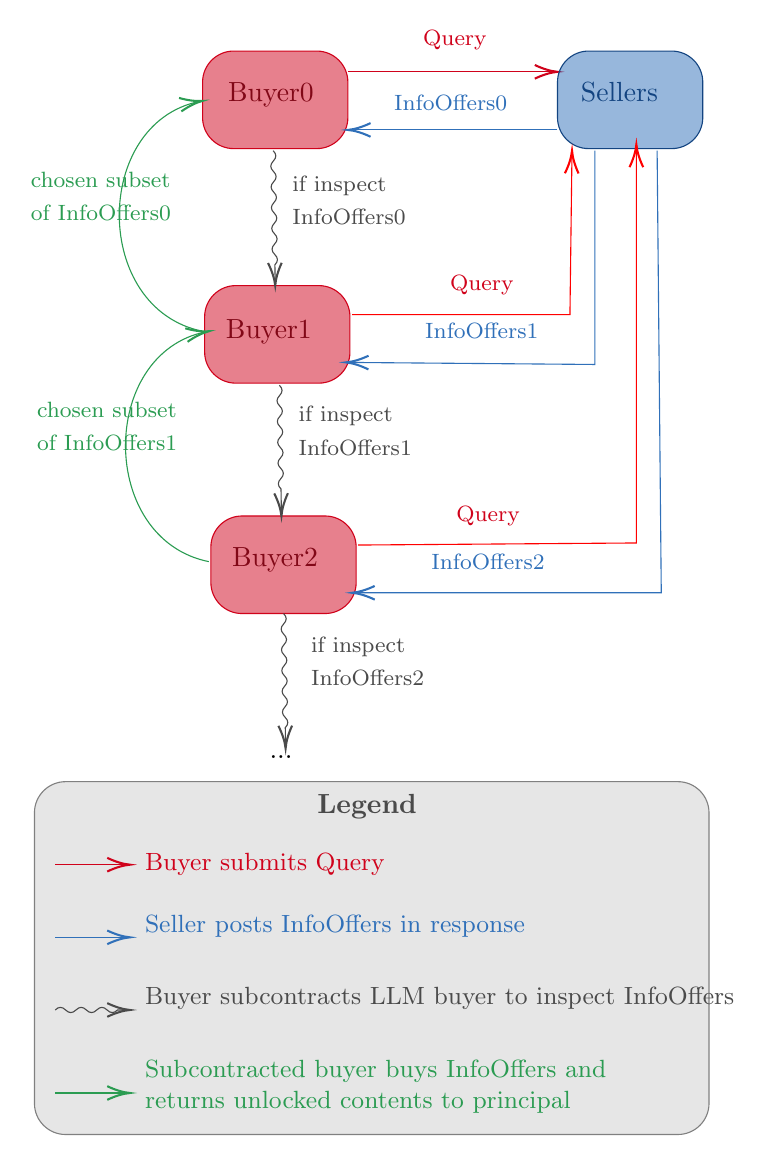
\begin{tikzpicture}[x=0.75pt,y=0.75pt,yscale=-1,xscale=1]
%uncomment if require: \path (0,439); %set diagram left start at 0, and has height of 439

%Straight Lines [id:da41524339668881804]
\draw [color={rgb, 255:red, 208; green, 2; blue, 27 }  ,draw opacity=1 ]   (161,43) -- (260,43) ;
\draw [shift={(262,43)}, rotate = 180] [color={rgb, 255:red, 208; green, 2; blue, 27 }  ,draw opacity=1 ][line width=0.75]    (10.93,-3.29) .. controls (6.95,-1.4) and (3.31,-0.3) .. (0,0) .. controls (3.31,0.3) and (6.95,1.4) .. (10.93,3.29)   ;
%Shape: Rectangle [id:dp2007096083409725]
\draw  [color={rgb, 255:red, 208; green, 2; blue, 27 }  ,draw opacity=1 ][fill={rgb, 255:red, 208; green, 2; blue, 27 }  ,fill opacity=0.5 ] (91,48) .. controls (91,39.72) and (97.72,33) .. (106,33) -- (146,33) .. controls (154.28,33) and (161,39.72) .. (161,48) -- (161,65) .. controls (161,73.28) and (154.28,80) .. (146,80) -- (106,80) .. controls (97.72,80) and (91,73.28) .. (91,65) -- cycle ;
%Shape: Rectangle [id:dp9891337920473939]
\draw  [color={rgb, 255:red, 19; green, 68; blue, 129 }  ,draw opacity=1 ][fill={rgb, 255:red, 48; green, 112; blue, 185 }  ,fill opacity=0.5 ] (262,48) .. controls (262,39.72) and (268.72,33) .. (277,33) -- (317,33) .. controls (325.28,33) and (332,39.72) .. (332,48) -- (332,65) .. controls (332,73.28) and (325.28,80) .. (317,80) -- (277,80) .. controls (268.72,80) and (262,73.28) .. (262,65) -- cycle ;
%Straight Lines [id:da08286653243829956]
\draw [color={rgb, 255:red, 48; green, 112; blue, 185 }  ,draw opacity=1 ]   (262,71) -- (163,71) ;
\draw [shift={(161,71)}, rotate = 360] [color={rgb, 255:red, 48; green, 112; blue, 185 }  ,draw opacity=1 ][line width=0.75]    (10.93,-3.29) .. controls (6.95,-1.4) and (3.31,-0.3) .. (0,0) .. controls (3.31,0.3) and (6.95,1.4) .. (10.93,3.29)   ;
%Shape: Rectangle [id:dp12709317008599474]
\draw  [color={rgb, 255:red, 208; green, 2; blue, 27 }  ,draw opacity=1 ][fill={rgb, 255:red, 208; green, 2; blue, 27 }  ,fill opacity=0.5 ] (92,161) .. controls (92,152.72) and (98.72,146) .. (107,146) -- (147,146) .. controls (155.28,146) and (162,152.72) .. (162,161) -- (162,178) .. controls (162,186.28) and (155.28,193) .. (147,193) -- (107,193) .. controls (98.72,193) and (92,186.28) .. (92,178) -- cycle ;
%Straight Lines [id:da9212547384246598]
\draw [color={rgb, 255:red, 74; green, 74; blue, 74 }  ,draw opacity=1 ]   (125,81) .. controls (126.69,82.64) and (126.72,84.31) .. (125.08,86) .. controls (123.44,87.69) and (123.46,89.35) .. (125.15,91) .. controls (126.84,92.64) and (126.87,94.31) .. (125.23,96) .. controls (123.59,97.69) and (123.62,99.36) .. (125.31,101) .. controls (127,102.65) and (127.02,104.31) .. (125.38,106) .. controls (123.74,107.69) and (123.77,109.36) .. (125.46,111) .. controls (127.15,112.64) and (127.18,114.31) .. (125.54,116) .. controls (123.9,117.69) and (123.93,119.36) .. (125.62,121) .. controls (127.31,122.64) and (127.33,124.3) .. (125.69,125.99) .. controls (124.05,127.68) and (124.08,129.35) .. (125.77,130.99) .. controls (127.46,132.63) and (127.49,134.3) .. (125.85,135.99) -- (125.85,136) -- (125.97,144) ;
\draw [shift={(126,146)}, rotate = 269.12] [color={rgb, 255:red, 74; green, 74; blue, 74 }  ,draw opacity=1 ][line width=0.75]    (10.93,-3.29) .. controls (6.95,-1.4) and (3.31,-0.3) .. (0,0) .. controls (3.31,0.3) and (6.95,1.4) .. (10.93,3.29)   ;
%Curve Lines [id:da5955388933274229]
\draw [color={rgb, 255:red, 43; green, 156; blue, 82 }  ,draw opacity=1 ]   (91,168) .. controls (37.54,157.11) and (37.99,67.81) .. (89.43,57.29) ;
\draw [shift={(91,57)}, rotate = 170.36] [color={rgb, 255:red, 43; green, 156; blue, 82 }  ,draw opacity=1 ][line width=0.75]    (10.93,-3.29) .. controls (6.95,-1.4) and (3.31,-0.3) .. (0,0) .. controls (3.31,0.3) and (6.95,1.4) .. (10.93,3.29)   ;
%Shape: Rectangle [id:dp3154829905272625]
\draw  [color={rgb, 255:red, 208; green, 2; blue, 27 }  ,draw opacity=1 ][fill={rgb, 255:red, 208; green, 2; blue, 27 }  ,fill opacity=0.5 ] (95,272) .. controls (95,263.72) and (101.72,257) .. (110,257) -- (150,257) .. controls (158.28,257) and (165,263.72) .. (165,272) -- (165,289) .. controls (165,297.28) and (158.28,304) .. (150,304) -- (110,304) .. controls (101.72,304) and (95,297.28) .. (95,289) -- cycle ;
%Straight Lines [id:da3417537956466643]
\draw [color={rgb, 255:red, 74; green, 74; blue, 74 }  ,draw opacity=1 ]   (128,194) .. controls (129.69,195.64) and (129.72,197.31) .. (128.08,199) .. controls (126.44,200.69) and (126.47,202.36) .. (128.16,204) .. controls (129.85,205.64) and (129.88,207.31) .. (128.24,209) .. controls (126.6,210.69) and (126.63,212.36) .. (128.32,214) .. controls (130.01,215.64) and (130.04,217.31) .. (128.4,219) .. controls (126.76,220.69) and (126.79,222.36) .. (128.48,224) .. controls (130.17,225.64) and (130.2,227.31) .. (128.56,229) .. controls (126.92,230.69) and (126.94,232.35) .. (128.63,233.99) .. controls (130.32,235.63) and (130.35,237.3) .. (128.71,238.99) .. controls (127.07,240.68) and (127.1,242.35) .. (128.79,243.99) -- (128.84,247) -- (128.97,255) ;
\draw [shift={(129,257)}, rotate = 269.09] [color={rgb, 255:red, 74; green, 74; blue, 74 }  ,draw opacity=1 ][line width=0.75]    (10.93,-3.29) .. controls (6.95,-1.4) and (3.31,-0.3) .. (0,0) .. controls (3.31,0.3) and (6.95,1.4) .. (10.93,3.29)   ;
%Curve Lines [id:da391924904621877]
\draw [color={rgb, 255:red, 43; green, 156; blue, 82 }  ,draw opacity=1 ]   (94,279) .. controls (40.54,268.11) and (40.99,178.81) .. (92.43,168.29) ;
\draw [shift={(94,168)}, rotate = 170.36] [color={rgb, 255:red, 43; green, 156; blue, 82 }  ,draw opacity=1 ][line width=0.75]    (10.93,-3.29) .. controls (6.95,-1.4) and (3.31,-0.3) .. (0,0) .. controls (3.31,0.3) and (6.95,1.4) .. (10.93,3.29)   ;
%Straight Lines [id:da3637784039757481]
\draw [color={rgb, 255:red, 74; green, 74; blue, 74 }  ,draw opacity=1 ]   (130,304) .. controls (131.69,305.64) and (131.72,307.31) .. (130.08,309) .. controls (128.44,310.69) and (128.46,312.35) .. (130.15,314) .. controls (131.84,315.64) and (131.87,317.31) .. (130.23,319) .. controls (128.59,320.69) and (128.62,322.36) .. (130.31,324) .. controls (132,325.65) and (132.02,327.31) .. (130.38,329) .. controls (128.74,330.69) and (128.77,332.36) .. (130.46,334) .. controls (132.15,335.64) and (132.18,337.31) .. (130.54,339) .. controls (128.9,340.69) and (128.93,342.36) .. (130.62,344) .. controls (132.31,345.64) and (132.33,347.3) .. (130.69,348.99) .. controls (129.05,350.68) and (129.08,352.35) .. (130.77,353.99) .. controls (132.46,355.63) and (132.49,357.3) .. (130.85,358.99) -- (130.85,359) -- (130.97,367) ;
\draw [shift={(131,369)}, rotate = 269.12] [color={rgb, 255:red, 74; green, 74; blue, 74 }  ,draw opacity=1 ][line width=0.75]    (10.93,-3.29) .. controls (6.95,-1.4) and (3.31,-0.3) .. (0,0) .. controls (3.31,0.3) and (6.95,1.4) .. (10.93,3.29)   ;
%Straight Lines [id:da5447878474416243]
\draw [color={rgb, 255:red, 255; green, 0; blue, 0 }  ,draw opacity=1 ]   (163,160) -- (268,160) -- (268.97,83) ;
\draw [shift={(269,81)}, rotate = 90.73] [color={rgb, 255:red, 255; green, 0; blue, 0 }  ,draw opacity=1 ][line width=0.75]    (10.93,-3.29) .. controls (6.95,-1.4) and (3.31,-0.3) .. (0,0) .. controls (3.31,0.3) and (6.95,1.4) .. (10.93,3.29)   ;
%Straight Lines [id:da3778704064531401]
\draw [color={rgb, 255:red, 255; green, 0; blue, 0 }  ,draw opacity=1 ]   (166,271) -- (300,270) -- (300,80) ;
\draw [shift={(300,78)}, rotate = 90] [color={rgb, 255:red, 255; green, 0; blue, 0 }  ,draw opacity=1 ][line width=0.75]    (10.93,-3.29) .. controls (6.95,-1.4) and (3.31,-0.3) .. (0,0) .. controls (3.31,0.3) and (6.95,1.4) .. (10.93,3.29)   ;
%Straight Lines [id:da28955812841585316]
\draw [color={rgb, 255:red, 48; green, 112; blue, 185 }  ,draw opacity=1 ]   (280,81) -- (280,184) -- (162,183.02) ;
\draw [shift={(160,183)}, rotate = 0.48] [color={rgb, 255:red, 48; green, 112; blue, 185 }  ,draw opacity=1 ][line width=0.75]    (10.93,-3.29) .. controls (6.95,-1.4) and (3.31,-0.3) .. (0,0) .. controls (3.31,0.3) and (6.95,1.4) .. (10.93,3.29)   ;
%Straight Lines [id:da7668238798267074]
\draw [color={rgb, 255:red, 48; green, 112; blue, 185 }  ,draw opacity=1 ]   (310,81) -- (312,294) -- (165,294) ;
\draw [shift={(163,294)}, rotate = 360] [color={rgb, 255:red, 48; green, 112; blue, 185 }  ,draw opacity=1 ][line width=0.75]    (10.93,-3.29) .. controls (6.95,-1.4) and (3.31,-0.3) .. (0,0) .. controls (3.31,0.3) and (6.95,1.4) .. (10.93,3.29)   ;

%Shape: Legend Rectangle [id:dp5647832748705617] - repositioned below diagram
\draw  [color={rgb, 255:red, 128; green, 128; blue, 128 }  ,draw opacity=1 ][fill={rgb, 255:red, 155; green, 155; blue, 155 }  ,fill opacity=0.25 ] (10,400) .. controls (10,391.72) and (16.72,385) .. (25,385) -- (320,385) .. controls (328.28,385) and (335,391.72) .. (335,400) -- (335,540) .. controls (335,548.28) and (328.28,555) .. (320,555) -- (25,555) .. controls (16.72,555) and (10,548.28) .. (10,540) -- cycle ;

% Legend Title
\draw (145,390) node [anchor=north west][inner sep=0.75pt]  [color={rgb, 255:red, 74; green, 74; blue, 74 }  ,opacity=1 ] [align=left] {\textbf{Legend}};

% Legend Row 1, Item 1: Red arrow - Buyer submits Query
\draw [color={rgb, 255:red, 208; green, 2; blue, 27 }  ,draw opacity=1 ]   (20,425) -- (54,425) ;
\draw [shift={(56,425)}, rotate = 180] [color={rgb, 255:red, 208; green, 2; blue, 27 }  ,draw opacity=1 ][line width=0.75]    (10.93,-3.29) .. controls (6.95,-1.4) and (3.31,-0.3) .. (0,0) .. controls (3.31,0.3) and (6.95,1.4) .. (10.93,3.29)   ;
\draw (62,418) node [anchor=north west][inner sep=0.75pt]  [font=\small,color={rgb, 255:red, 208; green, 2; blue, 27 }  ,opacity=1 ] [align=left] {Buyer submits Query};

% Legend Row 1, Item 2: Blue arrow - Seller posts InfoOffers
\draw [color={rgb, 255:red, 48; green, 112; blue, 185 }  ,draw opacity=1 ]   (54,460) -- (20,460) ;
\draw [shift={(56,460)}, rotate = 180] [color={rgb, 255:red, 48; green, 112; blue, 185 }  ,draw opacity=1 ][line width=0.75]    (10.93,-3.29) .. controls (6.95,-1.4) and (3.31,-0.3) .. (0,0) .. controls (3.31,0.3) and (6.95,1.4) .. (10.93,3.29)   ;
\draw (62,448) node [anchor=north west][inner sep=0.75pt]  [font=\small,color={rgb, 255:red, 48; green, 112; blue, 185 }  ,opacity=1 ] [align=left] {Seller posts InfoOffers in response};

% Legend Row 2, Item 1: Gray wavy arrow - Buyer subcontracts
\draw [color={rgb, 255:red, 74; green, 74; blue, 74 }  ,draw opacity=1 ]   (20,495) .. controls (21.67,493.33) and (23.33,493.33) .. (25,495) .. controls (26.67,496.67) and (28.33,496.67) .. (30,495) .. controls (31.67,493.33) and (33.33,493.33) .. (35,495) .. controls (36.67,496.67) and (38.33,496.67) .. (40,495) .. controls (41.67,493.33) and (43.33,493.33) .. (45,495) .. controls (46.67,496.67) and (48.33,496.67) .. (50,495) -- (54,495) ;
\draw [shift={(56,495)}, rotate = 180] [color={rgb, 255:red, 74; green, 74; blue, 74 }  ,draw opacity=1 ][line width=0.75]    (10.93,-3.29) .. controls (6.95,-1.4) and (3.31,-0.3) .. (0,0) .. controls (3.31,0.3) and (6.95,1.4) .. (10.93,3.29)   ;
\draw (62,483) node [anchor=north west][inner sep=0.75pt]  [font=\small,color={rgb, 255:red, 74; green, 74; blue, 74 }  ,opacity=1 ] [align=left] {Buyer subcontracts LLM buyer to inspect InfoOffers};

% Legend Row 2, Item 2: Green arrow - Subcontracted buyer buys
\draw [color={rgb, 255:red, 43; green, 156; blue, 82 }  ,draw opacity=1 ]   (20,535) -- (54,535) ;
\draw [shift={(56,535)}, rotate = 180] [color={rgb, 255:red, 43; green, 156; blue, 82 }  ,draw opacity=1 ][line width=0.75]    (10.93,-3.29) .. controls (6.95,-1.4) and (3.31,-0.3) .. (0,0) .. controls (3.31,0.3) and (6.95,1.4) .. (10.93,3.29)   ;
\draw (62,518) node [anchor=north west][inner sep=0.75pt]  [font=\small,color={rgb, 255:red, 43; green, 156; blue, 82 }  ,opacity=1 ] [align=left] {Subcontracted buyer buys InfoOffers and\\returns unlocked contents to principal};
% Text Node
\draw (102,47) node [anchor=north west][inner sep=0.75pt]  [color={rgb, 255:red, 129; green, 8; blue, 23 }  ,opacity=1 ] [align=left] {Buyer0};
% Text Node
\draw (272,47) node [anchor=north west][inner sep=0.75pt]  [color={rgb, 255:red, 19; green, 68; blue, 129 }  ,opacity=1 ] [align=left] {Sellers};
% Text Node
\draw (196,22) node [anchor=north west][inner sep=0.75pt]  [color={rgb, 255:red, 208; green, 2; blue, 27 }  ,opacity=1 ] [align=left] {{\footnotesize Query}};
% Text Node
\draw (182,53) node [anchor=north west][inner sep=0.75pt]  [color={rgb, 255:red, 48; green, 112; blue, 185 }  ,opacity=1 ] [align=left] {{\footnotesize InfoOffers0}};
% Text Node
\draw (101,161) node [anchor=north west][inner sep=0.75pt]  [color={rgb, 255:red, 129; green, 8; blue, 23 }  ,opacity=1 ] [align=left] {Buyer1};
% Text Node
\draw (133,92) node [anchor=north west][inner sep=0.75pt]  [color={rgb, 255:red, 74; green, 74; blue, 74 }  ,opacity=1 ] [align=left] {{\footnotesize if inspect}\\{\footnotesize InfoOffers0}};
% Text Node
\draw (209,140) node [anchor=north west][inner sep=0.75pt]  [color={rgb, 255:red, 208; green, 2; blue, 27 }  ,opacity=1 ] [align=left] {{\footnotesize Query}};
% Text Node
\draw (197,163) node [anchor=north west][inner sep=0.75pt]  [color={rgb, 255:red, 48; green, 112; blue, 185 }  ,opacity=1 ] [align=left] {{\footnotesize InfoOffers1}};
% Text Node
\draw (7,90) node [anchor=north west][inner sep=0.75pt]  [color={rgb, 255:red, 43; green, 156; blue, 82 }  ,opacity=1 ] [align=left] {{\footnotesize chosen subset}\\{\footnotesize of InfoOffers0}};
% Text Node
\draw (104,271) node [anchor=north west][inner sep=0.75pt]  [color={rgb, 255:red, 129; green, 8; blue, 23 }  ,opacity=1 ] [align=left] {Buyer2};
% Text Node
\draw (136,203) node [anchor=north west][inner sep=0.75pt]  [color={rgb, 255:red, 74; green, 74; blue, 74 }  ,opacity=1 ] [align=left] {{\footnotesize if inspect}\\{\footnotesize InfoOffers1}};
% Text Node
\draw (212,251) node [anchor=north west][inner sep=0.75pt]  [color={rgb, 255:red, 208; green, 2; blue, 27 }  ,opacity=1 ] [align=left] {{\footnotesize Query}};
% Text Node
\draw (200,274) node [anchor=north west][inner sep=0.75pt]  [color={rgb, 255:red, 48; green, 112; blue, 185 }  ,opacity=1 ] [align=left] {{\footnotesize InfoOffers2}};
% Text Node
\draw (10,201) node [anchor=north west][inner sep=0.75pt]  [color={rgb, 255:red, 43; green, 156; blue, 82 }  ,opacity=1 ] [align=left] {{\footnotesize chosen subset}\\{\footnotesize of InfoOffers1}};
% Text Node
\draw (142,314) node [anchor=north west][inner sep=0.75pt]  [color={rgb, 255:red, 74; green, 74; blue, 74 }  ,opacity=1 ] [align=left] {{\footnotesize if inspect}\\{\footnotesize InfoOffers2}};
% Text Node
\draw (122,371) node [anchor=north west][inner sep=0.75pt]   [align=left] {...};


\end{tikzpicture}

  }
  \caption{The Recursive Inspection Protocol}
  \label{fig:rim}
\end{figure}

\begin{figure}[htbp]
  \centering
  \begin{subfigure}[b]{\columnwidth}
    \centering
    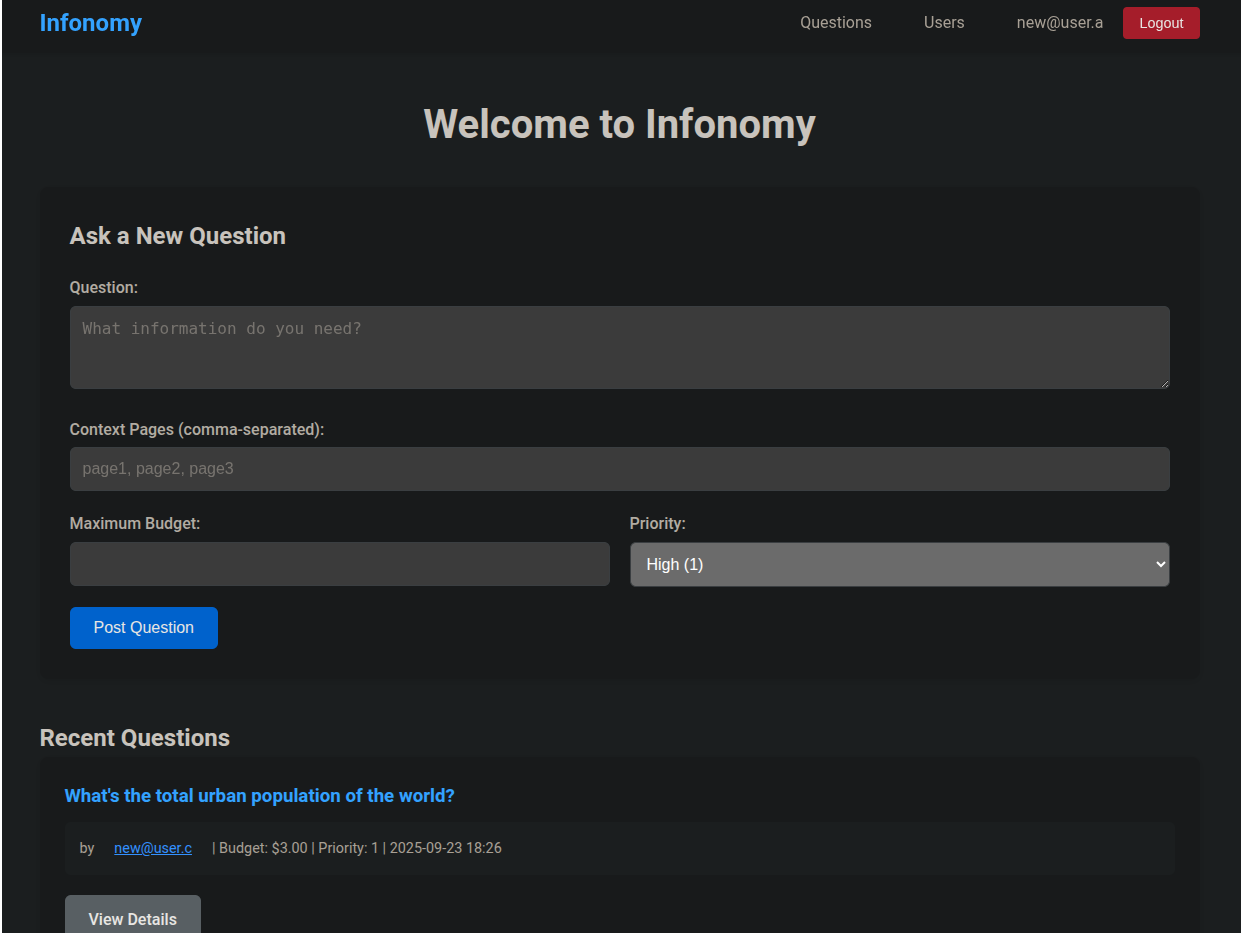
\includegraphics[width=0.9\linewidth]{figures/recursive-markets/infonomy_1.png}
    \caption{Posting a new question (\BuyerContext); viewing \BuyerContexts on the server}
    \label{fig:infonomy-1}
  \end{subfigure}

  \begin{subfigure}[b]{\columnwidth}
    \centering
    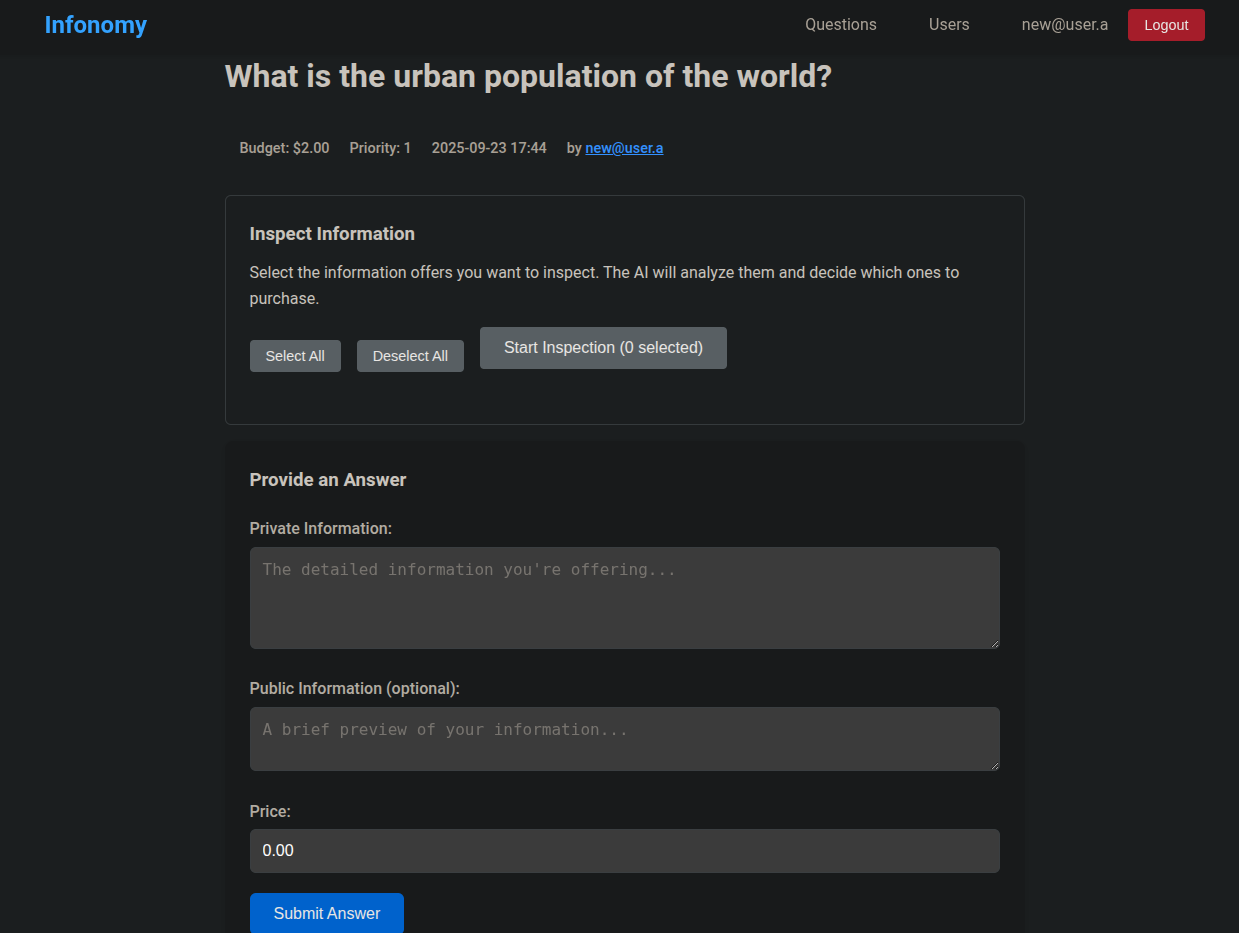
\includegraphics[width=0.9\linewidth]{figures/recursive-markets/infonomy_2.png}
    \caption{Posting an answer (\InfoOffer{}); initiating a recursive inspection}
    \label{fig:infonomy-2}
  \end{subfigure}

\end{figure}

\begin{figure}[htbp]
  \ContinuedFloat
  \centering
  \begin{subfigure}[b]{\columnwidth}
    \centering
    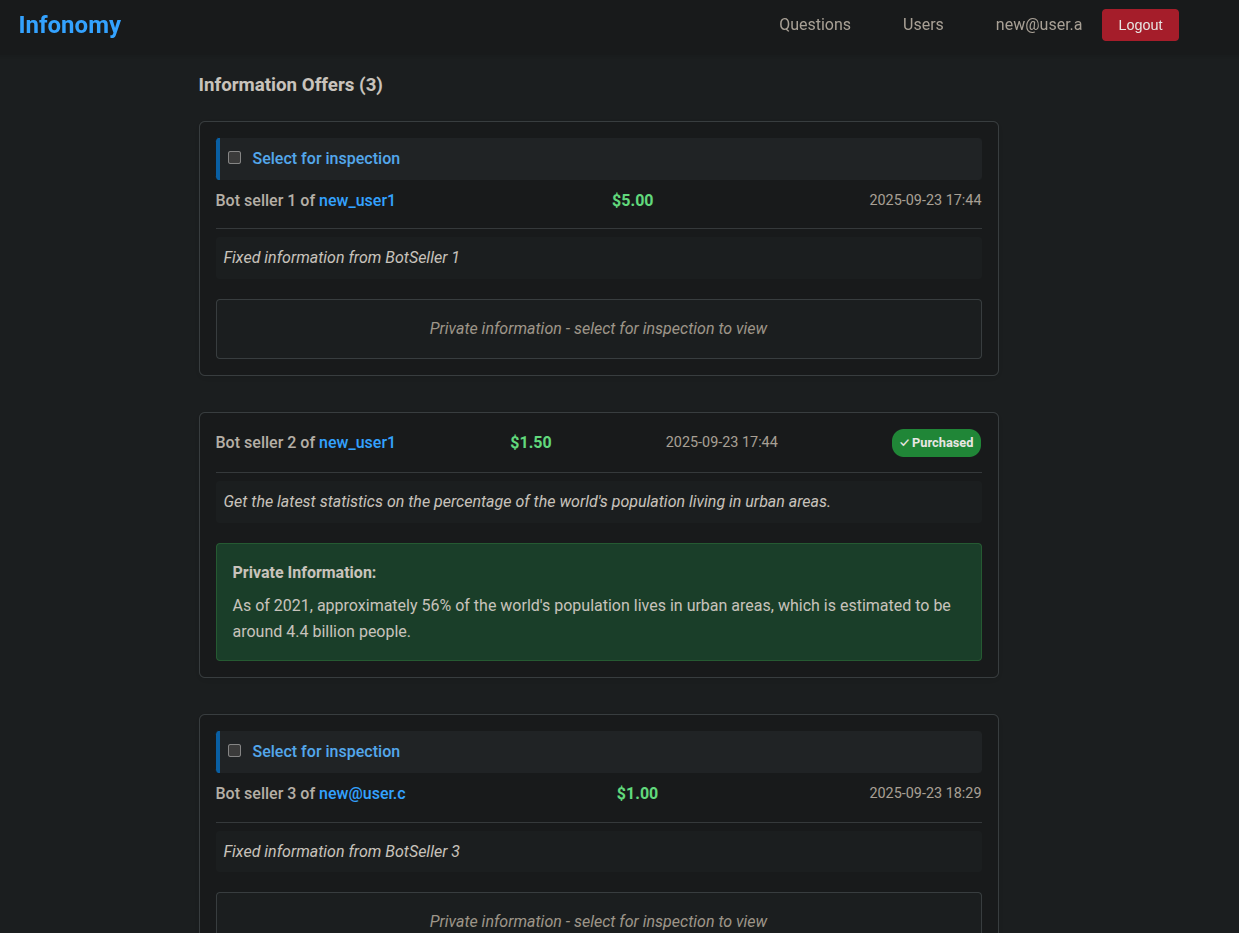
\includegraphics[width=0.9\linewidth]{figures/recursive-markets/infonomy_3.png}
    \caption{Inspecting and purchasing \InfoOffers{}; viewing purchased \InfoOffers{}}
    \label{fig:infonomy-3}
  \end{subfigure}

  \begin{subfigure}[b]{\columnwidth}
    \centering
    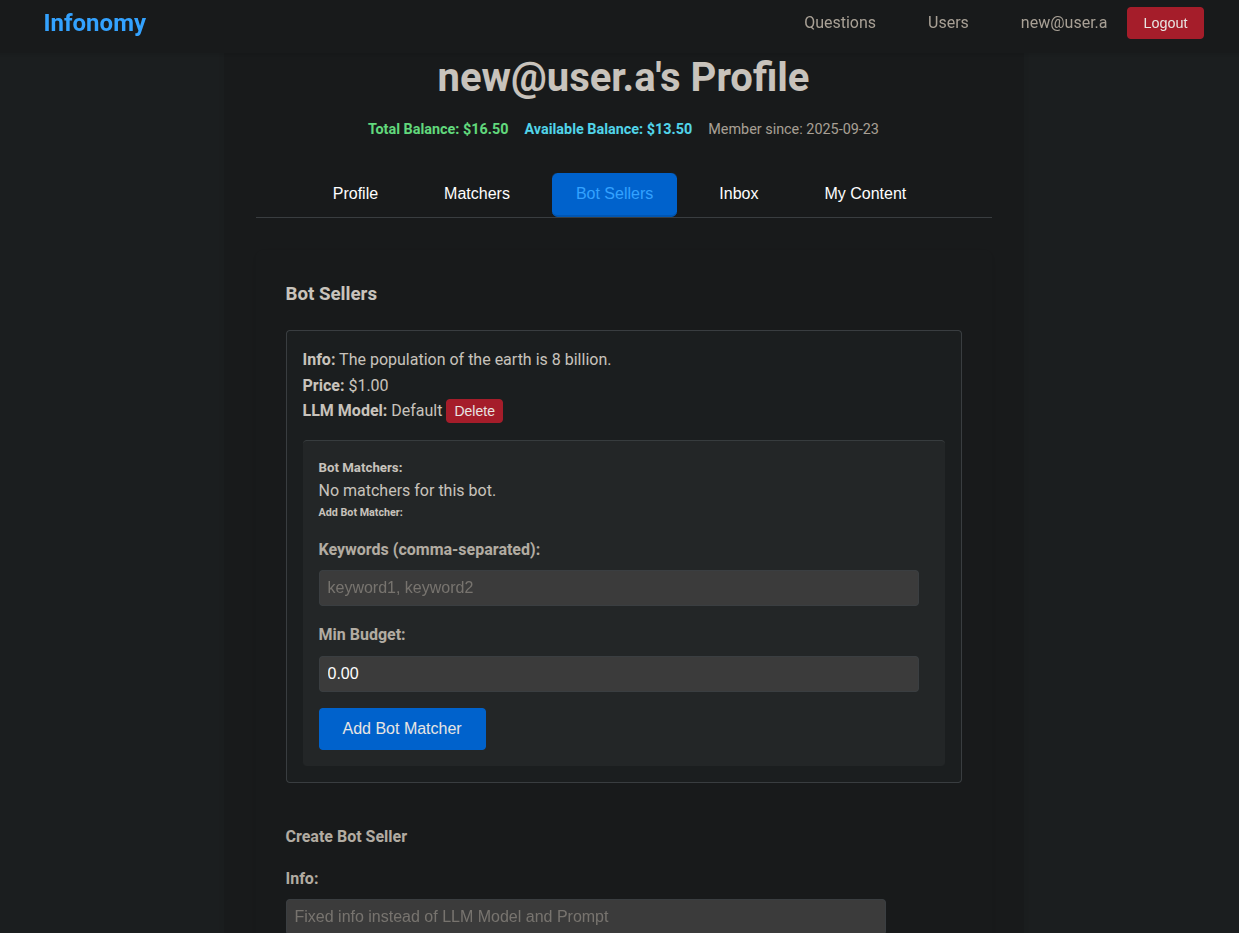
\includegraphics[width=0.9\linewidth]{figures/recursive-markets/infonomy_4.png}
    \caption{Bot sellers automatically answer recursive \BuyerContexts}
    \label{fig:infonomy-4}
  \end{subfigure}

  \caption{Screenshots from the \texttt{infonomy-server} platform}
  \label{fig:infonomy}
\end{figure}


A working implementation of an information market server implementing the Recursive Inspection Protocol is available at the \infonomy{} repository\footnote{\infonomyurl} -- some screenshots of the platform's GUI are shown in \Cref{fig:infonomy}. Many applications of such a server are immediate:

\begin{itemize}
\item \emph{Question \& Answer site} -- As presented, \infonomy{} can be seen as a Q \& A site with market incentives for answering questions.
\item \emph{Privatized product regulation} -- The \BuyerContexts{} might be names or links to products (the decision being ``should I buy?''), and the \InfoOffers{} could be inspection checks done by private labs, or customer reviews, which are now incentivized to be answerable to the customer.
\item \emph{Community Notes} -- In the spirit of well-known crowdsourced fact-checking systems such as Community Notes/Birdwatch \citeps{birdwatch2022}, we might use information markets as a ``comments section for the internet'', where \BuyerContexts{} would be links to webpages or social media posts (the decision being ``should I believe?'') and the \InfoOffers{} would be fact-checks or important context.
\item \emph{Reasoning in prediction markets} -- Forecasters on prediction markets may benefit from incentivizing the provision of information relevant to a forecast. One solution to this was given by \citets{conitzerPredictionMarketsMechanism2012}; another is to use \infonomy{}: where the \BuyerContexts{} are the questions being forecasted on (``What is the correct probability of this question?'') and the \InfoOffers{} are any relevant pieces of information.
\end{itemize}



\section{Future work}
\label{sec:so}

We have introduced a Bayesian framework for ``extrapolated volition'': i.e. to model a subjective buyer/rater's ``most fully informed'' score for the value of some piece of information. This allows us to design mechanisms for information markets (\cref{app:nonnaive}) as well as for supplying human feedback to AI models (\cref{sec:scoring}).

The ideal desideratum we would like a scalable oversight mechanism to satisfy is that it should incentivize the AI/information-seller to give the optimal information according to the information \emph{it} possesses: if the seller has information $K=(I_1,I_2,\dots)$, it should give information $I$ that optimizes\footnote{Naively one may think this means the AI should simply give $K$---realistically though, $K$ would be very large, reflecting the AI's entire knowledge and capabilities. Thus taking the cost of $K$ into account (assumed to be $\infty$ in \cref{sec:scoring}), that would certainly not be optimal.} $\mathbf{E}[U^1(I)|K=k]$. This would exactly describe the buyer's extrapolated volition: \emph{what would the buyer do if she were as smart as the AI?} Or we could say: this would exactly \emph{align} the AI or information-seller to our own values, while maintaining its superior information.

Unfortunately, our marginal value mechanism does not satisfy this hope. Take the following example.

\begin{example}
Suppose our decision problem is $\{0,1\}$ and:
\begin{itemize}
\item in our prior judgement, 0 is the better choice: $\mathbf{E}[U(0)]=1$, $\mathbf{E}[U(1)]=0$
\item  $I_1$ tells us 1 is better: $\mathbf{E}[U(0)|I_1]=0$, $\mathbf{E}[U(1)|I_1]=1$
\item  $I_2$ refutes $I_1$ and says 0 is better: $\mathbf{E}[U(0)|I_1,I_2]=1$ and $\mathbf{E}[U(1)|I_1,I_2]=0$
\item  $I_3$ refutes $I_2$ and says 1 is better: $\mathbf{E}[U(0)|I_1,I_2,I_3]=0$ and $\mathbf{E}[U(1)|I_1,I_2,I_3]=1$
\item with the full information, 1 is the better choice: $\mathbf{E}[U(0)|K]=0$, $\mathbf{E}[U(1)|K]=1$
\end{itemize}

But say $I_1$ and $I_2$ are cheap, while $p(I_3)=100$. Then the best information to reveal is $I_1$ --- but it won't be revealed, because $I_2$ will cheaply refute it while defending it with $I_3$ is too expensive. Thus instead we want to say that the agent can't give information \emph{so bad} that its shortfall exceeds its ``cost of defense'' (in this case, 100).

\end{example}

So while it is \emph{not} generally true that $x^1_*=\arg\max_{x^1}\mathbf{E}[U^1(x^1)|K]$, we may hope for a lower bound on ``how bad'' the equilibrium could possibly get, i.e. a result like $\mathbf{E}[U^1(x^1_*)|K]\ge \max_{x^1}\mathbf{E}[U^1(x^1)|K]-\mathcal{E}$ for some shortfall expression $\mathcal{E}$ that is some measure of the ``cost of defending the correct information''---and we may also use the expression for such a shortfall as a measure of how good a particular scalable oversight protocol is.


% We have introduced the \emph{recursive inspection protocol} as an information market mechanism for agents that are capable of ``inspecting and forgetting'' information, and provided a working implementation of the algorithm employing LLM agents. Our mechanism is optimal in a certain fundamental sense that accounts for the cost of obtaining information.

% The most promising direction for future work is to explore applications of this mechanism to \emph{scalable oversight} in AI alignment. Our mechanism may be seen as a formalization of Extrapolated Volition \citeps{yudkowskyCoherentExtrapolatedVolition2004}, which is informally described as the ``action an agent would prefer if it had all the relevant information''.
% \Cref{alg:rim} itself may be remniscient of scalable oversight proposals such as ``Humans Consulting HCH'' \citeps{christianoHCH}.

% More generally, one of the key limitations of currently widely-used alignment techniques such as reinforcement learning from human feedback (RLHF) is that they fundamentally rely on a human's ability to judge the correctness or value of a (potentially superhuman) AI's outputs \citeps{rlhflimits,burnsWeaktoStrongGeneralizationEliciting2024}. In other words, the AI is trained on the human supervisor's \emph{immediate, superficial} volition, rather than on her \emph{extrapolated volition} \citeps{yudkowskyCoherentExtrapolatedVolition2004}. In this context, our proposal may be used to augment a human rater's judgement of the AI's outputs with an information market, better reflecting her ``extrapolated volition''.
